\chapter{Números comlejos} \label{complejos}

\begin{tikzpicture}
	\fill [left color=red!50, right color=teal!50] (0,0) rectangle (6.5,.2);
	\fill [left color=teal!50, right color=blue!50] (6.5,0) rectangle (11.5,.2);
	\end{tikzpicture}



\vspace{10mm}


\begin{adjustwidth}{40pt}{40pt}
\begin{cuadro-gris}

	\begin{multicols}{2}
	$\triangleright \quad$   Necesidad de los números complejos, $\mathcal C$.
	
	$\triangleright \quad$   Forma binómica de un número complejo.
	
	$\triangleright \quad$   Formas trigonométrica y polar de un número complejo.
	
	$\triangleright \quad$   Potenciación y radicación en $\mathcal C$

	$\triangleright \quad$   Ecuaciones en $\mathcal C$
	
	\end{multicols}
	
\end{cuadro-gris}
\end{adjustwidth}


\vspace{.5cm}
\section{Necesidad de los números complejos}

\begin{tikzpicture}
	\fill [left color=red!50, right color=teal!50] (0,0) rectangle (3.5,.1);
	\fill [left color=teal!50, right color=blue!50] (3.5,0) rectangle (7.5,.1);
	\end{tikzpicture}
\vspace{0.5cm}



\begin{adjustwidth}{40pt}{40pt}
\begin{destacado}
\texttt{$\ $``... los números negativos no pueden tener raíces cuadradas. Pero supongamos que ...''$\ $}
\footnote{$\ $ La Historia de las Matemáticas en los últimos 10.000 años. Ian Stewart.}
\end{destacado}
\end{adjustwidth}

\vspace{0.5cm}
El nombre escogido para estos números tiene lo suyo, pero ... sigamos adelante.

Estos extraños números (los números complejos a que nos vamos a enfrentar) surgen de la mano de \emph{Cardano} y \emph{Tartaglia} en el \emph{s. XVI}, cuando intentaban resolver ecuaciones de tercer grado. Se dieron cuenta que necesitaban tener en cuanta a las raíces cuadradas de números negativos, así, p.e., lo que hacían para calcular $\sqrt{-25}$ era lo siguiente: $\ \sqrt{-25} = \sqrt{25\cdot (-1)}=\sqrt{25}\cdot \sqrt{-1}=5\cdot \sqrt{-1}$

En el \emph{s. XVII}, \emph{Leibniz} considera a la $\sqrt{-1}$ como una \emph{``especie de anfibio entre el ser y la nada''}. Los matemáticos y físicos de la época usan estos números pero con desconfianza.

\emph{Euler}, en el \emph{s. XVIII} bautiza a $\sqrt{-1}$ como $\boldsymbol i$, de número imaginario. Ahora, las raíces de números negativos son algo tan sencillo como $\pm \sqrt{-4}=\pm 2\, i$

A finales del \emph{s. XVIII}, \emph{Euler} demuestra su famoso \emph{TEOREMA FUNDAMENTAL DEL ÁLGEBRA}, que asegura que todo polinomio de grado $n$ tiene, exactamente, $n$-raíces. Así, p.e., la ecuación $x^2-4x+13=0$ tiene por soluciones $2+3i$ y $2-3i$ (compruébese).

A partir del \emph{s. XIX}, \emph{Gauss} logra la representación gráfica de estos números complejos y su interpretación geométrica. Desde entonces, los números complejos son aceptados sin reservas.

En la actualidad, la aplicación de los números complejos está presente en muchos apartados de las ciencias.
\begin{itemize}
\item En electrónica, que llaman $\boldsymbol j$ a la $\sqrt{-1}$ para no confundirla con la intensidad de corriente, la ley de \emph{Ohm} (IR=V) para corriente alterna necesita de los números complejos: IZ=V; Z=R+jX (Z impedancia, tiene parte real o resistiva R y parte imaginaria o reactancia X)
\item También se usan los números complejo en electromagnetismo (las ondas electromagnéticas son complejas) y en física cuántica (la amplitud de probabilidad es compleja, su cuadrado es lo observable).
\item En la teoría especial de la relatividad se reformula el espacio-tiempo 4-dimensional de \emph{Minkowski} en el que el tiempo es una componente más, imaginaria. En palabras de \emph{Minkowski}, en \emph{1908}, \emph{``las ideas que sobre el espacio-tiempo quiero mostrarles hoy descansan en el suelo firme de la física experimental, en la cual yace su fuerza. Son ideas radicales. Por lo tanto, el espacio y el tiempo, por separado, están destinados a desvanecerse entre las sombras y tan solo una unión de ambos puede representar la realidad''.}
\item Qué no decir de los fractales. En \emph{1977 Benoit Mandelbrot} publica \emph{``la geometría fractal de la naturaleza''}, regida por números complejos ($z_{n+1}=z_n^2+c$, conjunto de Mandelbrot).
\end{itemize}


\begin{figure}[H]
	\centering
	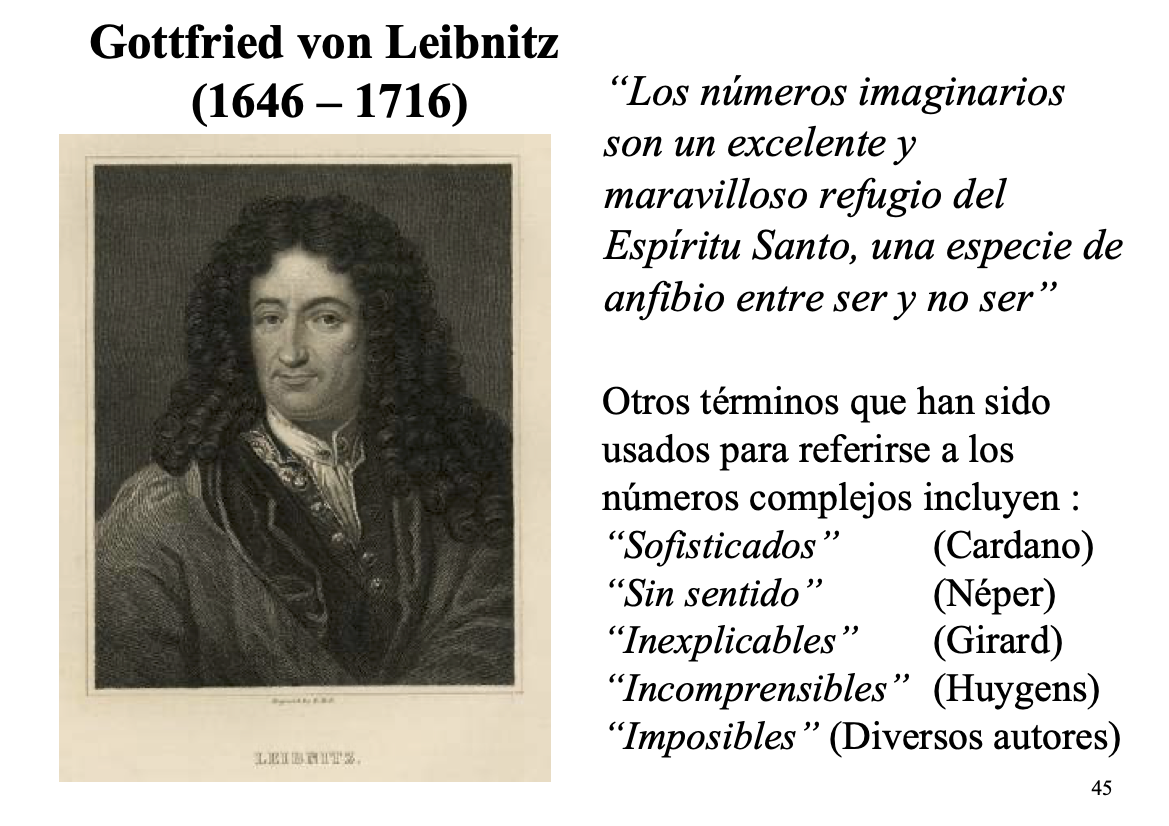
\includegraphics[width=0.85\textwidth]{img-c/comp06.png}
\end{figure}

\vspace{5mm}
\begin{myexampleblock}{Historia de los números complejos}
\begin{small}
Las ideas matemáticas revolucionarias rara vez se descubren en los contextos simples, casi siempre surgen de algo mucho más complicado. Así sucedió con la raíz cuadrada de menos uno. Hoy día, lo habitual es introducir este número en términos de la ecuación cuadrática $x2 + 1 =0$, cuya solución es la raíz cuadrada de menos uno, cualquier cosa que esto signifique.

\vspace{1mm} Entre los primeros matemáticos en preguntarse si eso de la raíz de menos uno tenía un sentido razonable estaban los algebristas del Renacimiento, que tropezaron con las raíces cuadradas de números negativos de una manera sorprendentemente indirecta: la solución de ecuaciones cúbicas.

\vspace{1mm} Scipione Del Ferro (1465-1526) y Niccolò Fontana (Tartaglia, 1499-1557) descubrieron soluciones algebraicas a las ecuaciones cúbicas, posteriormente expuestas por Girolamo Cardano (1501-1576) en su Ars Magna (Cardano consiguió, mediante adulaciones, que Tartaglia le enseñase su método para resolver ecuaciones cúbicas y lo publicó en 1545 a pesar de haberle jurado a Tartaglia que no lo difundiría). En símbolos modernos, la solución de una ecuación cubica $x^3 + ax = b$ es:

$$x \ = \ \sqrt[3]{ \, \dfrac b 2 \, + \, \sqrt{ \, \dfrac{a^3}{27} \, + \, \dfrac{b^2}{4} \, } \, }  \ + \ 
\sqrt[3]{ \, \dfrac b 2 \, - \, \sqrt{ \, \dfrac{a^3}{27} \, + \, \dfrac{b^2}{4} \, } \, } $$

Los matemáticos del Renacimiento expresaban esta solución en palabras, pero el procedimiento era el mismo.

\vspace{1mm} A veces esta formula funcionaba muy bien, pero otras veces tropezaba con problemas. Cardano advirtió que cuando la formula se aplica a la ecuación $x^3 -15x = 4$, que tiene la solución obvia $x = 4$ (evidentemente, $4^3-15\cdot 4=4$), el resultado se expresa como:

$$x\ = \ \sqrt[3]{2+\sqrt{-121}} \ + \ \sqrt[3]{2-\sqrt{-121}}$$

Sin embargo, esta expresión no parecía tener un significado razonable, porque -121 no tiene raíz cuadrada. Un Cardano intrigado escribió a Tartaglia pidiéndole una aclaración, pero la  respuesta  de Tartaglia fue inútil.

\vspace{1mm} Una respuesta, si así se le puede llamar, fue ofrecida por Rafael Bombelli (1526-1572) en su libro en tres volúmenes L’Algebra, impreso en Venecia en 1572. A Bombelli le preocupaba que el Ars Magna de Cardano era bastante oscura, y se propuso escribir algo más claro. El operaba sobre la molesta raíz cuadrada como si fuera un número ordinario, y advirtió que :

$$(2+\sqrt{-1})^3=2+\sqrt{-121} \ \Rightarrow \ \sqrt[3]{2+\sqrt{-121}}=2+\sqrt{-1}\, ; \quad \text{análogamente } \ 
\sqrt[3]{2-\sqrt{-121}}=2-\sqrt{-1}$$


\textcolor{gris}{$\scriptsize{ 
\mqty{
(2+\sqrt{-1})^3=2^3+3\cdot 2^2 \sqrt{-1}+3\cdot 2 (\sqrt{-1})^2+(\sqrt{-1})^3=8+12\sqrt{-1}-6-\sqrt{-1} 
=2+11\sqrt{-1}=2+\sqrt{(-1)11^2}=2+\sqrt{-121} }
} $}


\vspace{3mm}Así, este extraño método daba la respuesta correcta, un entero perfectamente normal, pero al que se llegaba manipulando cantidades ``imposibles''.

\vspace{1mm} Para responder a por qué funcionan estas ideas, los matemáticos tuvieron que desarrollar buenas maneras de pensar en raíces cuadradas de cantidades negativas y hacer cálculos con ellas. Los autores anteriores, entre ellos Descartes y Newton, interpretaban estos números ``imaginarios'' como una señal de que un problema no tenía solución. Si uno quería encontrar un número cuya raíz cuadrada era menos uno, la solución formal ``raíz cuadrada de menos uno'' era imaginaria, de modo que no existía solución. Pero el cálculo de Bombelli implicaba que en los números imaginarios había algo más que eso, podían utilizarse para encontrar soluciones, podían ocurrir cuando las soluciones sí existían.

\vspace{1mm} En 1673 John Wallis inventó una manera sencilla de representar números imaginarios como puntos en un plano. Partió de la representación familiar de los números reales como una recta, con los números positivos a la derecha y los negativos a la izquierda. Luego introdujo otra recta, que formaba un ángulo recto con la primera, y colocó los imaginarios a lo largo de esta nueva recta. Esto es similar a la aproximación algebraica de Descartes a la geometría plana, utilizando ejes de coordenadas. Los números reales forman un eje en la figura, y los imaginarios otro. El resto del plano corresponde a números ``complejos'' que constan de dos partes: una real y una imaginaria.

\vspace{1mm} En coordenadas cartesianas medimos la parte real a lo largo de la recta real y medimos la parte imaginaria paralela a la recta imaginaria. Así, 3 + 2i yace tres unidades a la derecha del origen y dos unidades arriba. La idea de Wallis resolvía el problema de dar sentido a los números imaginarios, pero nadie le prestó la más mínima atención. No obstante, su idea ganó terreno lentamente en el subconsciente de los matemáticos. La mayoría de ellos dejaron de preocuparse porque la raíz cuadrada de menos uno no pudiera ocupar una posición en la recta real, y se dieron cuenta de que podía vivir en algún lugar en el mundo más amplio del plano complejo. Algunos no apreciaron la idea: en 1758 François Daviet de Foncenex, en un artículo sobre números imaginarios, afirmaba que era absurdo pensar que los imaginarios formaban una recta a un ángulo recto con la recta real. Pero otros la tomaron en serio y entendieron su importancia.

\vspace{1mm} La idea de que un plano complejo podía ampliar la confortable recta real y dar hogar a los imaginarios estaba implícita en la obra de Wallis, aunque ligeramente oscurecida por la forma en que la presentaba. Fue explicitada por el noruego Caspar Wessel en 1797. Wessel era topógrafo, y lo que le interesaba principalmente era representar la geometría del plano en términos de números. En retrospectiva, sus ideas podían verse como un método de representar números complejos en términos de geometría plana. Pero él publicaba en danés, y su trabajo pasó desapercibido hasta un siglo más tarde, cuando fue traducido al francés. El matemático francés Jean-Robert Argand publicó independientemente la misma representación de los números complejos en 1806, y Gauss la describió independientemente de ambos en 1811.
\end{small}	
\end{myexampleblock}


\begin{figure}[H]
	\centering
	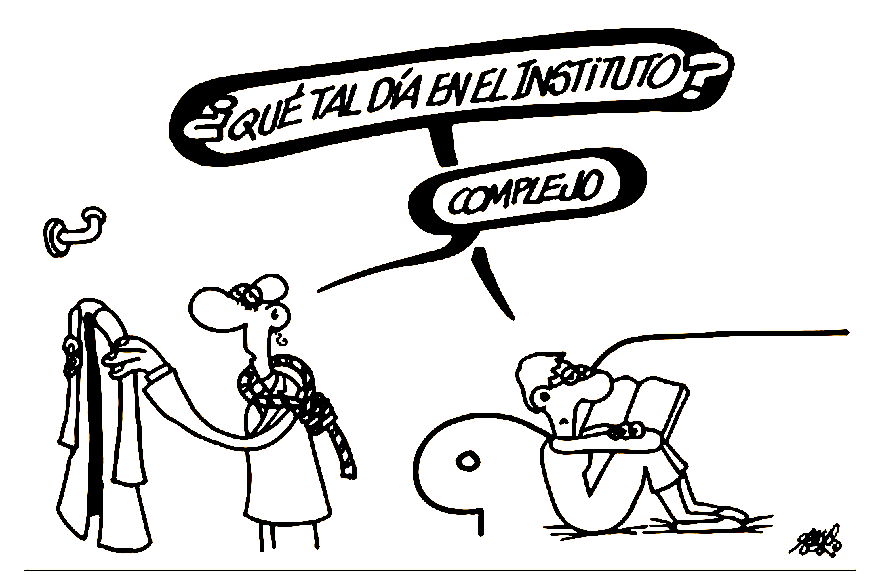
\includegraphics[width=0.75\textwidth]{img-c/comp01.png}
\end{figure}



\vspace{0.5cm}

\subsection{Unidad imaginaria. Potencias de $\boldsymbol i$}

\begin{tikzpicture}
	\fill [left color=red!50, right color=teal!50] (0,0) rectangle (3.5,.01);
	\fill [left color=teal!50, right color=blue!50] (3.5,0) rectangle (7.5,.01);
	\end{tikzpicture}
\vspace{0.5cm}


\begin{definition}[ Número $\boldsymbol i$ ]

Se define la \emph{unidad imaginaria}, 	$\boldsymbol i$, como:
$\qquad \boxed{ \ \subrayado{\boldsymbol {
i\ = \ \sqrt{-1}
}} \ } $
\end{definition}

\begin{definition}[ Número complejo]

Se denine un número complejo como
$\quad z\in \mathbb C\ \to \ z \ = \ a\ + \ b\, i \, ; \quad a, b \in \mathbb R$	

\vspace{2mm}donde, $a=\Re(z);\ b=\Im(z)$ son, respectivamente, las partes real e imaginaria del número complejo $z$. Obviamente, $\Re(z), \Im(z) \in \mathbb R$
\end{definition}

\begin{theorem}[ Sucesivas potencia de $\boldsymbol i$ ]

Solo existen cuatro potencias distintas de 	$\boldsymbol i$

\begin{table}[H]
\center
\begin{tabular}{lll}
$\boldsymbol i$ & $\quad$ & $\boldsymbol i^5=i^4\cdot i=i$ \\
$\boldsymbol i^2=\boldsymbol{ -1}$ &  & $\boldsymbol i^6=i^4\cdot i^2=i^2=-1$ \\
$\boldsymbol i^3=i^2\cdot i=- \boldsymbol{ i}$ &  & $\boldsymbol i^7=i^4\cdot i^3=i^3=-i$ \\
$\boldsymbol i^4=i^2\cdot i^2=(-1)\cdot (-1)=\boldsymbol 1$ &  & $\boldsymbol i^8=i^4\cdot i^4=i^4=1$
\end{tabular}
\end{table}

Solo aparecen como resultados $\quad \{i,\ -1,\ -i,\ 1\}$

% Please add the following required packages to your document preamble:
% \usepackage{multirow}
\begin{table}[H]
\center
\begin{tabular}{cccc}
\multicolumn{1}{c|}{n} & 4 & $\qquad$ & \multirow{2}{*}{$\boldsymbol{i^{n}=i^{4c+r}=i^{4c}\cdot i^r= (i^4)^c\cdot i^r=i^r }\, , \quad r=\{0,1,2,3\} $} \\ \cline{2-2}
r                      & c &         &                                                                 
\end{tabular}
\end{table}
$\boxed{\ \subrayado{\  i^0=1,\ i^1=i,\ i^2=-1;\ i^3=-i;\ i^4=1;\ } \ \ i^n=i^r,\ \small{ r=\{0,1,2,3\}\  \text{ resto de dividir } n \text{ entre }  4 } \ }$
\end{theorem}

\begin{miejemplo}

$$i^{47}=i^{4\cdot 11+3}=(i^4)^{11}	\cdot i^3=1^{11}\cdot i^3=i^3=-i$$
\end{miejemplo}

\begin{miejemplo}

Resuelve la ecuación $\quad x^2+8x+25=0$

\vspace{4mm} $\qquad x=\dfrac{-8\pm \sqrt{64-4\cdot 25}}{2}=\dfrac{-8\pm \sqrt{-36}}{2}=\dfrac{-8\pm 6\, \sqrt{-1}}{2}=\dfrac{-8\pm 6\, i}{2}=-4\pm 3\, i$	
\end{miejemplo}


\begin{definition}[ El conjunto de los números complejos]

$$\mathcal C \ = \ \{ z=x+i\, y \,; \  \ x,y \in \mathcal R \}\, ; \qquad x=\Re(z) \in \mathbb R\, ; \ y=\Im(z)\in \mathbb R$$
\end{definition}

Así definido el conjunto de los números complejos hace que los números reales sean un subconjunto de ellos. 
Efectivamente, $\quad \forall x=\in \mathbb R \, , \ x=x+0\, i=z \in \mathbb C \ \Rightarrow \ \subrayado{ \boxed{ \ \boldsymbol{ \mathbb R \subset \mathbb C }\ } }  $

\begin{multicols}{2}
Los número reales son números complejos cuya parte imaginaria es cero.

$\quad$

Si la parte imaginaria no es cero, tenemos los `números imaginarios' o complejos. 

$\quad$

Aquellos números imaginarios cuya parte real es cero se llaman `imaginarios puros'.

$\quad$
	\begin{figure}[H]
	\centering
	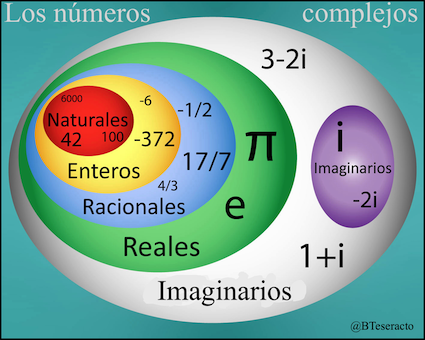
\includegraphics[width=0.45\textwidth]{img-c/comp05.png}
\end{figure}
\end{multicols}




\begin{definition}[ Igualdad de número complejos]

Dos números complejos son iguales si tienen las mismas partes reales y las mismas partes imaginarias:
$\qquad (z_1=a_1+b_1\, i)\, , (z_2=a_2+b_2\, i)\, \in \mathbb C\ : \qquad
\boldsymbol{
z_1=z_2 \ \leftrightarrow \ a_1=a_1 \ \wedge \ b_1=b_2
 }$ 
\end{definition}


\vspace{1cm}
\section{Forma binómica de un número complejo}

\begin{tikzpicture}
	\fill [left color=red!50, right color=teal!50] (0,0) rectangle (3.5,.1);
	\fill [left color=teal!50, right color=blue!50] (3.5,0) rectangle (7.5,.1);
	\end{tikzpicture}
\vspace{0.5cm}


La forma de escribir los números complejos que hemos visto hasta ahora recibe el nombre de \emph{``forma binónica''} o rectangular.
$\qquad  z\in \mathbb C\ \to \ z \ = \ a\ + \ b\, i \, ; \quad a=\Re(z)\, , b=\Im(z)\,  \in \,  \mathbb  R$

\begin{multicols}{2}
$\quad$

De este modo, los número complejos admiten una representación en el plano: \emph{\textbf{Diagrama de Argand}} o \emph{\textbf{plano complejo}}. Se representan en el eje de las $x$ (abcisas) la parte real de $z$ y en el de las $y$ (ordenadas) se representa la parte imaginaria.

\begin{figure}[H]
	\centering
	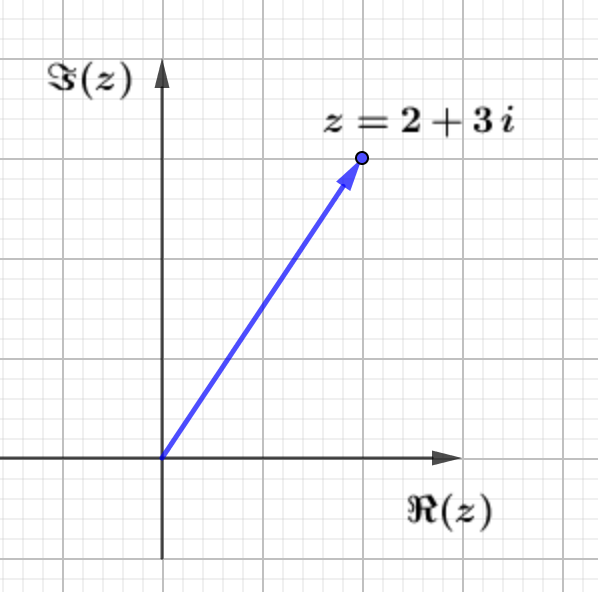
\includegraphics[width=0.3\textwidth]{img-c/comp02.png}
\end{figure}
\end{multicols}

\begin{definition}[ Conjugado de un número complejo]

Dado un número complejo $z\ $, se llama \emph{\textbf{complejo conjugado}} y se representa por $\bar z$, al número	complejo que resulta de cambiar de signo a la parte imaginaria.

$$z=a+b\, i \, \in \, \mathbb C  \quad \to \quad  \bar z=\ \overline{a+b\, i} \ = a-b\,i \ \in \mathbb C$$

Evidentemente, $\ \overline{\bar z}\ = z$
\end{definition}



\subsection{Operaciones de complejos en forma binómica}

\vspace{5mm}
\textbf{Producto de un número real por un número complejo}

$$z=a+b\, i \, \in \, \mathbb C\, ; \ \ k \in \mathbb R \quad \to \quad k\cdot z=k\cdot a + k\cdot b\, i \ \in \mathbb C$$

Para multiplicar un número real por un número complejo, se multiplican las partes reales e imaginarias del número complejo por el número real.

\vspace{5mm}
\textbf{Suma de números complejos}

$z_1=a_1+b_1\, i\, , \ z_2=a_2+b_2\, i\,  \quad \to \quad
z_1+z_2 \ =  (a_1+b_1\, i)+(a_2+b_2\, i)=\  (a_1+a_2) \ + \ (b_1+b_2)\, i$

\begin{destacado}
La suma de dos números complejos es otro número complejo cuya parte real es la suma de partes reales y la parte imaginaria es la suma de las partes imaginarias.
\end{destacado}

\vspace{5mm}
\textbf{Resta de números complejos}

\begin{definition}[ Opuesto de un número complejo]

Dado $z=a+b\, i \ \in \mathbb C$, el opuesto de $z$, que representaremos por $-z$, se obtiene como producto del número complejo $z$ por el número real $(-1):\qquad \boldsymbol{-z\ = \ (-1) \cdot z}$	
\end{definition}

\begin{destacado}
Restar dos números complejos es sumar al primero de ellos el opuesto del segundo: \end{destacado}

$\boldsymbol{z_1-z_2=z_1+(-1)\cdot z_2}; \qquad \qquad z_1-z_2=(a_1+b_1\, i)-(a_2-b_2\, i)=(a_1-a_2)+(b_1-b_2)\, i$

Al igual que para los números reales, la suma de números complejos cumple las propiedades asociativa y conmutativa. El neutro de la suma de números complejos es el número complejo $0=0+ 0 \, i$

\vspace{5mm}
\textbf{Productos de números complejos}

\begin{destacado}
Dados  $z_1=a_1+b_1\, i\, , \ z_2=a_2+b_2\, i \ \in \mathbb C \ $ se define el producto de dos números complejos como el producto de estos dos binomios teniendo en cuenta que $i^2=-1$.\end{destacado}

$z_1\cdot z_2 \ =  (a_1+b_1\, i)\cdot (a_2+b_2\, i)=a_1a_2+a_1b_2\, i+b_1a_2\, i+b_1b_2 \cancelto{-1}{i^2}=(a_1a_2-b_1b_2)+(a_1b_2+a_2b_1)\, i\ \in \mathbb C$  

Al igual que para los números reales, el producto de números complejos cumple las propiedades asociativa y conmutativa. El neutro del producto de números complejos es el número complejo $1=1+ 0 \, i\, . \ $ También se cumple la propiedad distributiva del producto respecto de la suma de complejos. \textcolor{gris}{$[\, z_1\cdot (z_2+z_3)=z_1\cdot z_2+z_1\cdot z_3 \, ]$}

\vspace{5mm}
\begin{theorem}[ Producto de un complejo por su conjugado]

El producto de un complejo por su complejo conjugado en un número real igual a la parte real al cuadrado más la parte imaginaria al cuadrado.

$$z=a+b\, i \ \in \mathbb C \quad \Rightarrow \quad z\cdot \bar z=a^2+b^2 \in \mathbb R$$	
\end{theorem}

\underline{Demostración}: $\quad  z=a+b\, i \ \in \mathbb C \ \to \ \bar z=a-b\, i \ \Rightarrow$

$\Rightarrow \quad  z\cdot \bar z=(a+bi)\cdot(a-bi)=a^2+ \cancel{ab\, i}- \cancel{ab\, i}-b^2\, \cancelto{-1}{i^2}=a^2+b^2 \ \in \mathbb R$ \QED

\vspace{5mm}
\begin{definition}[ Inverso de un número complejo] 

Dado $z=a+b\, i \ \in \mathbb C$, el inverso de $z$, que representaremos por $z^{-1}=\dfrac{1}{z}$, se obtiene multiplicando numerador y denominador por el complejo conjugado de $z$ 

$$z^{-1}=\dfrac 1 z = \dfrac 1 z \cdot \dfrac{\bar z}{\bar z}=\dfrac{\bar z}{z\cdot \bar z}= \dfrac{a-b\, i}{a^2+b^2}= \dfrac{a}{a^2+b^2}+ \dfrac{-b}{a^2+b^2}\, i \ \in \mathbb C$$	
	
\end{definition}

\vspace{5mm}
\textbf{División de números complejos}

\begin{destacado}
Para dividir dos números complejos, multiplicaremos numerador y denominador por el complejo conjugado del denominador.\end{destacado}

$z_1=a_1+b_1\, i\, , \ z_2=a_2+b_2\, i \ \in \mathbb C \ \to \ $

$$\to \quad 
\subrayado{\boxed{ \ \boldsymbol{ \dfrac{z_1}{z_2}=\dfrac{z_1}{z_2} \cdot \dfrac{\bar z_2}{\bar z_2} } \ }}= \dfrac{(a_1+b_1\, i)(a_2-b_2\, i)}{(a_2+b_2\, i)(a_2-b_2\ i)}=
\dfrac{a_1a_1+b_1b_2}{a_2^2+b_2^2}+\dfrac{-a_1b_2+a_2b_1}{a_2^2+b_2^2}\, i \ \in \mathbb C$$


\begin{miejemplo}

Calcula: $\qquad a)\ (2+3\, i)(3-4\, i);\qquad b)\ \dfrac{2+3\, i}{3-4\, i}$

\vspace{6mm} $\triangleright \quad a)\ \  (2+3\, i)(3-4\, i)=6-8\, i+9\, i-12\, i^2=6-8\, i+9\, i+12=18+\, i$


\vspace{4mm} $\triangleright \quad b)\ \	 \dfrac{2+3\, i}{3-4\, i}=\dfrac{(2+3\, i)(3+4\, i)}{(3-4\, i)(3+4\, i)}=\dfrac{6+8\, i+9\, i+12\, i^2}{9-16\, i^2}=\dfrac{-6+17\, i}{25}= \dfrac{-6}{25}+\dfrac{17}{25}\, i$
\end{miejemplo}


\begin{miejercicio}

Calcula: $\qquad a)\ (1+i)^4;\qquad b)\ i^{-1}$	

\rule{250pt}{0.5pt}

\vspace{2mm} $\triangleright \quad a)\ \ (1+i)^4=\mqty(4\\0)\ 1^4+\mqty(4\\1)\ 1^3\, i+\mqty(4\\2)\ 1^2 \, \cancelto{-1}{i^2}+\mqty(4\\3)\ 1\, \cancelto{-i}{i^3}+\mqty(4\\4) \ \cancelto{1}{i^4}=$

\vspace{2mm}$=1+4\, i+ 6\, (-1)+4 (-i)+1=-4$


\vspace{4mm} $\triangleright \quad b)\ \ i^{-1}=\dfrac 1 i = \dfrac{1\cdot (-i)}{i\cdot (-i)}=\dfrac{-i}{-(\cancelto{-1}{i^2})}=\dfrac{-i}{+1}=-i$




\end{miejercicio}

\begin{theorem} [ Potencias enteras negativas de $\boldsymbol i$	]

Sabemos que $i^2=-1;\quad i^3=-i;\quad i^4=1\ $ y acabamos de ver que $i^{-1}=-i$, por lo que:

\vspace{2mm} $i^{-2}=i^{-1}\cdot i^{-1}=(-i)(-i)=i^2=-1;\qquad i^{-3}=i^{-2}\cdot i^{-1}=(-1)(-i)=i;\qquad i^{-4}=i^{-3}\cdot i^{-1}=i(-i)=-i^2=+1 \ $ y a partir de ahora se repiten los resultados obtenidos $\ \{-i,-1,i,\ 1\}$ 

\vspace{4mm}  En general, $\quad \boxed{\  \boldsymbol{ i^{-n}=\ \dfrac{1}{i^n}=\left( \dfrac 1 i \right)^n=(-i)^n\ =(-1)^n\cdot i^n } \ }$ 
\end{theorem}



\begin{miejercicio}

Calcula $\  i^{-47}$

\rule{250pt}{0.5pt}

\vspace{2mm} De la fórmula anterior,  $\ i^{-47} =(-1)^{47}\cdot i^{47} \, , $ en el ejemplo 9.1 vimos $i^{47}=-i$, por lo que $\ i^{-47}=(-1)(-i)=+i$

\vspace{4mm} De otra forma, $\ i^{-47}=(i^{47})^{-1}= \small{ \text{ (ejemplo 9.1) } } =(-i)^3=-i^3=-(-i)=+i$
\end{miejercicio}




\vspace{1cm}
\section{Forma polar y trigonométrica de un número complejo}

\begin{tikzpicture}
	\fill [left color=red!50, right color=teal!50] (0,0) rectangle (3.5,.1);
	\fill [left color=teal!50, right color=blue!50] (3.5,0) rectangle (7.5,.1);
	\end{tikzpicture}
\vspace{0.5cm}

\begin{large} \textbf{Forma polar de un número complejo} \end{large}

Vamos a ver otra forma de escribir números complejos que es de mucha utilidad en productos y cocientes, ya que facilita mucho los cálculos.


\begin{multicols}{2}

$$r=\sqrt{a^2+b^2}=\sqrt{z\cdot \bar z}$$

$$\tan \theta=\dfrac b a $$

$$\subrayado{\boxed{ \  \boldsymbol{ z\ = \ a\ + \ b\, i \ = \ r_{\ \theta} } \ } }$$
	
\begin{figure}[H]
	\centering
	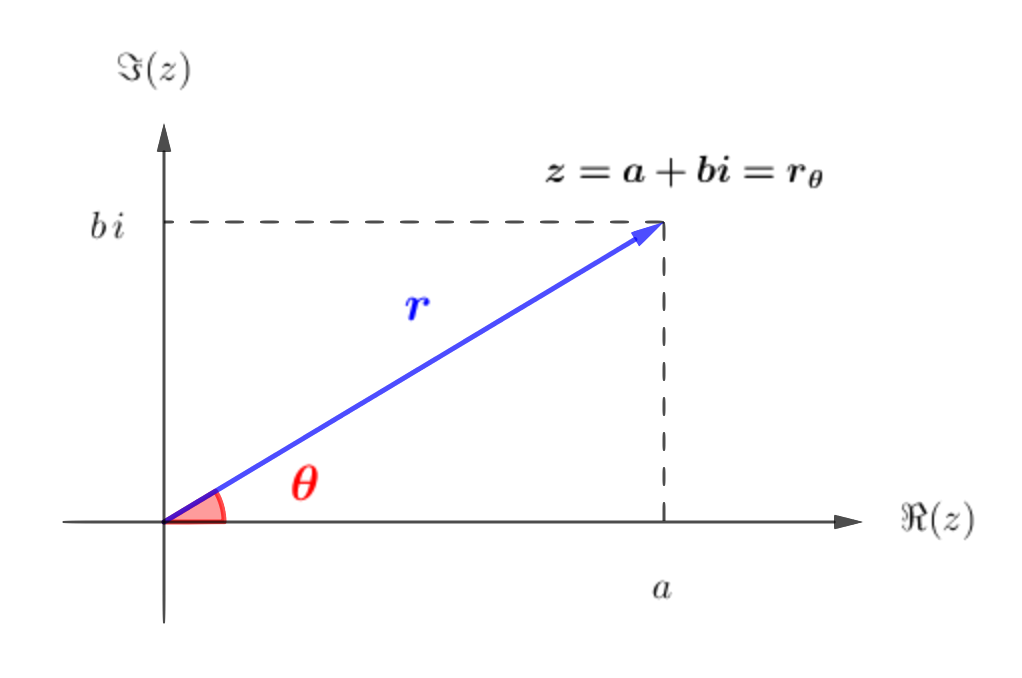
\includegraphics[width=0.5\textwidth]{img-c/comp04.png}
\end{figure}
\end{multicols}

\underline{Observaciones}:

\begin{itemize}
\item $\boldsymbol r$ es el \textbf{\emph{módulo}} del número complejo $z$, $\ r \in \mathbb R^+$ (el módulo es un número real no negativo, $ \ r\in [0,+\infty[$). Representa la distancia del $z$ al origen de coordenadas.

\item $\boldsymbol \theta$ es el \textbf{\emph{argumento}} del número complejo $z$, mide el ángulo que forma $\mathcal O z$ con el semieje $X$ positivo.

Como $\theta$ está definido como un arcotangente, $\ \theta =\atan \, (b/a) \, , \ $ el argumento no está bien definido pues cada numero complejo posee una infinidad de ellos ($\theta$ y $\theta+2k\pi,\ \forall k\in \mathbb Z$ tienen la misma tangente). Para solucionar este problema suele definirse lo que se llama \textbf{argumento principal} y tomar $\theta \in [0,2\pi[$; esto será lo que haremos en este nivel de matemáticas.
\end{itemize}

\vspace{10mm}
\begin{miejemplo}

Pasa a polar los números $\quad \pm 1\pm i$

\vspace{4mm} $\triangleright \quad \ \  1+i  \in \ \text{ primer cuadrante, } \theta \in [0,\pi/2[ \quad \to \ $	

\vspace{2mm} $r=\sqrt{1^2+1^2}=\sqrt{2};\quad \theta=\atan \dfrac{1}{1}=1 \to \begin{cases} \ \theta=45 \\ \ \cancel{\theta=225} \end{cases} \quad \Rightarrow \quad 1+i=\sqrt{2}_{\ 45^o}$


\vspace{4mm} $\triangleright \quad -1+i \in \text{ segundo cuadrante, }  \theta \in [\pi/2,\pi[  \quad \to \ $

\vspace{2mm} $r=\sqrt{(-1)^2+1^2}=\sqrt{2};\quad \theta=\atan \dfrac{1}{-1}=-1 \to \begin{cases} \ \theta=135 \\ \ \cancel{\theta=315} \end{cases} \quad \Rightarrow \quad -1+i=\sqrt{2}_{\ 135^o}$

\vspace{4mm} $\triangleright \quad -1-i \in \text{ tercer cuadrante, }  \theta \in [\pi,3\pi/2[ \quad \to \ $

\vspace{2mm} $r=\sqrt{(-1)^2+(-1)^2}=\sqrt{2};\quad \theta=\atan \dfrac{-1}{-1}=1 \to \begin{cases} \ \cancel{\theta=45} \\ \ \theta=225 \end{cases} \quad \Rightarrow \quad -1-i=\sqrt{2}_{\ 225^o}$

\vspace{4mm} $\triangleright \quad \ \ 1-i \in \ \text{ cuarto cuadrante, }  \theta \in [3\pi/2,2\pi[ \quad \to \ $	

\vspace{2mm} $r=\sqrt{1^2+(-1)^2}=\sqrt{2};\quad \theta=\atan \dfrac{-1}{1}=-1 \to \begin{cases} \ \cancel{\theta=135} \\ \ \theta=315  \end{cases} \quad \Rightarrow \quad 1-i=\sqrt{2}_{\ 315^o}$

\end{miejemplo}

\begin{miejercicio}

Pasa a forma polar: $\quad \sqrt{3}-i;\qquad 1+\sqrt{3}\, i$

\rule{250pt}{0.5pt}

\vspace{2mm} $\triangleright\quad  r=\sqrt{(\sqrt{3})^2+(-1)^2}=2;\ \ \theta=\atan \dfrac{-1}{\sqrt{3}}=-\dfrac{\sqrt{3}}{3} \to \begin{cases} \ \cancel{\theta=150} \\ \ \theta=330  \end{cases} \ \ \Rightarrow \ \  $

$\Rightarrow \ \  \sqrt{3}-i=2_{\ 330^o} \ {(3-cdte)}$	

\vspace{4mm} $\triangleright\quad r=\sqrt{1^2+(\sqrt{3})^2}=2;\ \ \theta=\atan \dfrac{\sqrt{3}}{1}=\sqrt{3}\ \  \to \ \ \begin{cases}  \ \theta=60 \\ \ \cancel{\theta=300}   \end{cases} \ \ \Rightarrow \ \  $

$\Rightarrow \ \  1+\sqrt{3}\, i=2_{\ 60^o} \ {(1-cdte)}$	

	
\end{miejercicio}

\vspace{5mm}
\begin{adjustwidth}{10pt}{10pt}
	\begin{cuadro-naranja}
		\emph{\textsf{Los números reales tienen por módulo su valor absoluto y por argumento $0$ ó $\pi=180^o$ según sean positivos o negativos, respectivamente. Los números imaginarios (imaginarios puros, aquellos cuya parte real es cero) tiene por módulo el valor absoluto de la parte imaginaria y por argumento $\pi/2=90^o$ o $3\pi/2=270^o$ según su parte imaginaria sea positiva o negativa, respectivamente.}}
	\end{cuadro-naranja}
\end{adjustwidth}

\begin{miejercicio}

Pasa a forma polar: $\quad 3,\ \ -4,\ \ 2\, i,\ \ -5 \, i$

\rule{250pt}{0.5pt}

\vspace{2mm} $\triangleright\quad  3\ $ es un número real que está a 3 u de distancia del origen y forma 0$^o$ con el eje $\mathcal OX$, por lo que: $\quad 3=3_{\ 0^o}$

\vspace{2mm} $\triangleright\quad  -3\ $ es un número real que está a 4 u de distancia del origen y forma 180$^o$ con el eje $\mathcal OX$, por lo que: $\quad -4=4_{\ 180^o}$

\vspace{2mm} $\triangleright\quad  2\, i \ $ es un número real que está a 2 u de distancia del origen y forma 90$^o$ con el eje $\mathcal OX$, por lo que: $\quad 2\, i=2_{\ 90^o}$

\vspace{2mm} $\triangleright\quad  -5\, i\ $ es un número real que está a 5 u de distancia del origen y forma 270$^o$ con el eje $\mathcal OX$, por lo que: $\quad -5\, i=5_{\ 270^o}$

\end{miejercicio}

\vspace{5mm} \begin{large} \textbf{Forma trigonométrica de un número complejo} \end{large}

De la misma definición de forma polar, podemos encontrar la forma binómica sin más que pasar por la forma trigonométrica:

\begin{multicols}{2}

$$x=r \cos \theta$$

$$y=r \sin \theta$$

$$\subrayado{\boxed{ \  \boldsymbol{ z\ = \ r_{\ \theta} \ = \ r\, \cos \theta \ + \ r \sin \theta \, i } \ } }$$
	
\begin{figure}[H]
	\centering
	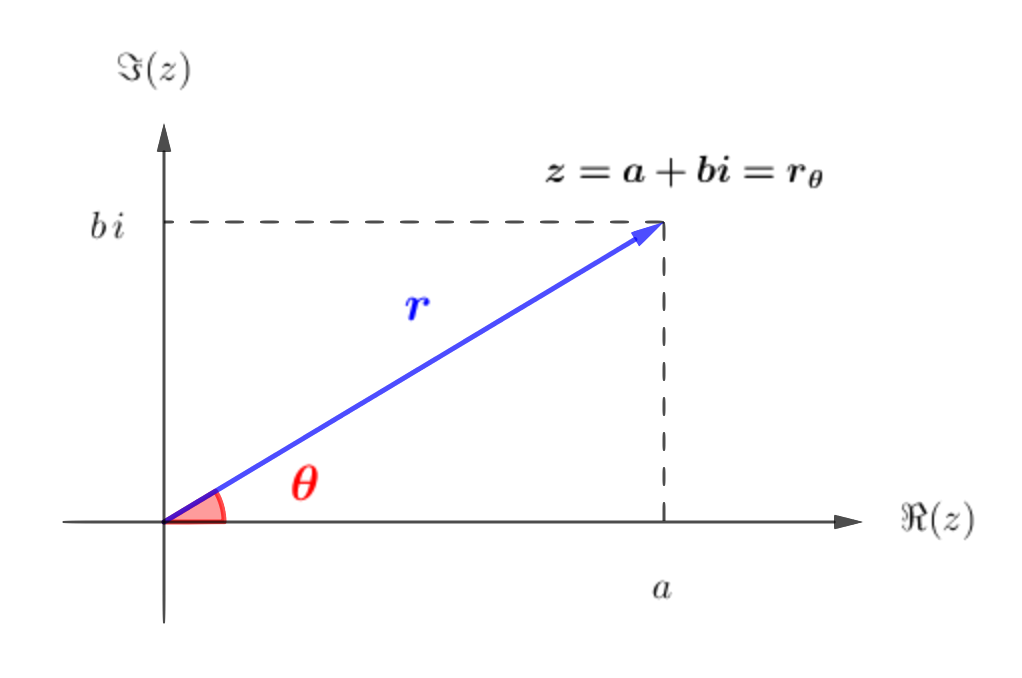
\includegraphics[width=0.5\textwidth]{img-c/comp04.png}
\end{figure}
\end{multicols}

\underline{Observaciones}:

\begin{itemize}
\item Se trata realmente de despejar en la forma polar para obtener la forma binómica: 

$ a=r\cos \theta ;\ \ b=r\sin \theta$	

\item $\qquad \subrayado{ \boxed{\ 
\boldsymbol{z \quad = \quad  
\underbrace {\ a \ + \ b\, i \ }_{\text{ forma binómica }} 
\quad = \quad 
\underbrace{\ r_{\ \theta} \ }_{\text{ forma polar }} 
\quad = \quad 
\underbrace{\ r\, (\cos \theta \ + \ \sin \theta \, i) \ }_{\text{ forma trigonométrica } } } 
\ } }$
\end{itemize}



\begin{myexampleblock}{ Simetrías en complejos}
	
	\begin{figure}[H]
	\centering
	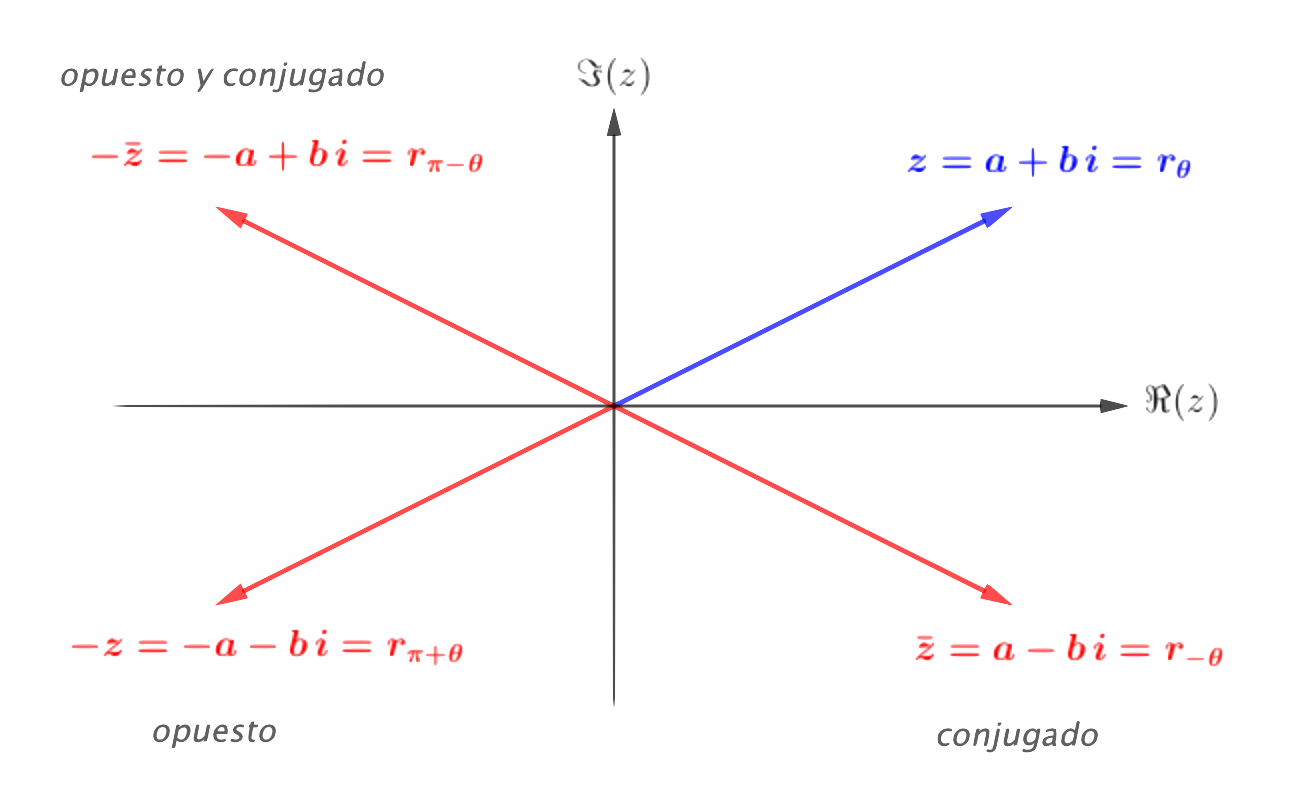
\includegraphics[width=1\textwidth]{img-c/comp03.png}
\end{figure}
\end{myexampleblock}



\subsection{Operaciones de complejos en forma polar}

\begin{tikzpicture}
	\fill [left color=red!50, right color=teal!50] (0,0) rectangle (3.5,.01);
	\fill [left color=teal!50, right color=blue!50] (3.5,0) rectangle (7.5,.01);
	\end{tikzpicture}
\vspace{0.5cm}

La forma polar simplifica mucho el cálculo en números complejos, sobre todo para productos y cocientes (y, claro está, en la potenciación y radicación como veremos más adelante del tema), pero no así para la suma y resta de complejos que seguiremos efectuando en forma binómica.

\vspace{5mm} \textbf{Producto de complejos en forma polar}

\begin{theorem}[ Producto de complejos en forma polar]

$$r_{\ \theta},\ s_{\ \varphi} \ \in \mathbb C \ \to \ \begin{cases}
 \ r_\theta=r\cos \theta+i\, r \sin \theta \\ \ s_\varphi	=s\cos \varphi +i\, s \sin \varphi  \end{cases} \ \Rightarrow \quad 
 \Large{ \subrayado{\boxed{\ \boldsymbol{r_{\ \theta} \, \cdot \, s_{\ \varphi} \ = \ (r\cdot s)_{\ \theta\, + \, \varphi}} \ }} }$$
 
El producto de  dos números complejos en  forma polar es un número complejo que tiene por módulo el producto de los módulos y por argumento la suma de los argumentos.

\end{theorem}

\underline{Demostración}:

$r_\theta \cdot s_\varphi=r\, (\cos \theta+i\, \sin \theta)\cdot  s\, (\cos \varphi+i\, \sin \varphi)= \ \textcolor{gris}{\ (i^2=-1)\ } \ =$

$=r\cdot s\ \left[ (\cos \theta \cos \varphi - \sin \theta \sin \varphi) \ + \ i\, (\sin \theta \cos \varphi + \cos \theta \sin \varphi) \right] =$

$=r\cdot s \ [ \, \cos (\theta+\varphi) \ + \ i\, \sin (\theta`\varphi)\, ] = (r\cdot s)_{\ \theta+\varphi}$ \QED

\vspace{5mm} \textbf{Cociente de complejos en forma polar}


\begin{theorem}[ Cociente de complejos en forma polar]

$$r_{\ \theta},\ s_{\ \varphi} \ \in \mathbb C \ \to \ \begin{cases}
 \ r_\theta=r\cos \theta+i\, r \sin \theta \\ \ s_\varphi	=s\cos \varphi +i\, s \sin \varphi  \end{cases} \ \Rightarrow \quad 
 \Large{ \subrayado{\boxed{\ \boldsymbol{
\dfrac{ r_{\ \theta} }{ \ s_{\ \varphi}} \ = \ \left( \dfrac r s \right)_{\ \theta\, - \, \varphi} 
 } \ }} }$$
 
 El cociente de  dos números complejos en  forma polar es un número complejo que tiene por módulo el cociente de los módulos y por argumento la resta de los argumentos.

\end{theorem}

\underline{Demostración}:

$\dfrac{ r_\theta }{ s_\varphi} = \dfrac{r\, (\cos \theta+i\, \sin \theta)} {s\, (\cos \varphi+i\, \sin \varphi)}=$
$\dfrac r s \ \dfrac{ (\cos \theta+i\, \sin \theta)}{ (\cos \varphi+i\, \sin \varphi)} \cdot \dfrac { (\cos \varphi-i\, \sin \varphi)}{ (\cos \varphi-i\, \sin \varphi)} = \ \textcolor{gris}{\ (i^2=-1)\ } \ =$

$=\dfrac r s \ \dfrac{\left[ (\cos \theta \cos \varphi + \sin \theta \sin \varphi) \ + \ i\, (\sin \theta \cos \varphi - \cos \theta \sin \varphi) \right]}{\cancelto{1}{\cos^2 \varphi + \sin^2 \varphi}} = $

$= \dfrac r s \ \left[ \, \cos (\theta-\varphi) \ + \ i\, \sin (\theta-\varphi)  \, \right] = \ \left( \dfrac r s \right)_{\ \theta-\varphi} $ \QED



\begin{miejemplo}

Calcula en forma polar y da el resultado en forma binómica: 

$a)\ \  2_{\ 150^o} \cdot \left( \dfrac 1 4 \right)_{\ 60^o}; \qquad  \qquad b)\ \ \left( \dfrac 1 3 \right)_{\ 150^o} \div 3_{\ 30^o}$

\vspace{4mm} $\triangleright \ \ a) \quad  2_{\ 150^o} \cdot \left( \dfrac 1 4 \right)_{\ 60^o} =\left( 2\cdot \dfrac 1 4 \right)_{150+60}= \left( \dfrac 1 2 \right)_{\ 210^o}= \dfrac 1 2 \, ( \cos 210^o + i\, \sin 210^o)=\dfrac 1 2 \ \left( -\dfrac{\sqrt{3}}{2} - i\, \dfrac 1 2   \right) =-\dfrac{\sqrt{3}}{4}-i\, \dfrac 1 4$

\vspace{4mm} $\triangleright \ \ b) \quad \left( \dfrac 1 3 \right)_{\ 150^o} \div 3_{\ 30^o} = \left( \dfrac 1 3 \div 3 \right)_{\ 150-30}=\left( \dfrac 1 9 \right)_{\ 120^o}=\dfrac 1 9 \, (cos 120^o+i\ \sin 120^o)=\dfrac 1 9 \left(-\dfrac 1 2 + i\ \dfrac{\sqrt{3}}{2} \right)= -\dfrac 1{18} + i\, \dfrac{\sqrt{3}}{18}$
	
\end{miejemplo}

\begin{miejercicio}

Dados $\ z_1=6_{\, 300^o},\ z_2=3\sqrt{2}_{\, 45^o},\ $ calcula:

\begin{multicols}{3}
\begin{enumerate}[a) ]
\item $z_1+z_2$
\item $z_1-z_2$
\item $\bar z_1$
\item $-z_2$
\item $z_1\cdot z_2$
\item $z_1 \div z_2$
\item $z_1\div z_2^2$	
\item $z_1^2\cdot \bar z_2$
\item $-z_1\cdot z_2$
\end{enumerate}
	
\end{multicols}


\rule{250pt}{0.1pt}

\vspace{4mm} $\triangleright \quad a)\ \ 6_{30}=6(\cos 30+i\sin 30)=3-3\sqrt{3}\ i;\quad 3\sqrt{2}_{45}=3\sqrt{2}(\cos 45+i\sin 45)=3+3 \, i$

\vspace{2mm} $z_1+z_2=3-3\sqrt{3}\ i \ + \ 3+3 \, i=6+3(1-\sqrt{3})\, i $

\vspace{6mm} $\triangleright \quad b)\ \ z_1-z_2=3-3\sqrt{3}\ i \ - \ (3+3 \, i)=-3(1+\sqrt{3})\, i$


\vspace{6mm} $\triangleright \quad c)\ \ \bar z_1=\overline{3-3\sqrt{3}\, i}=3+3\sqrt{3}\, i=6_{\, -300^o}=3_{\ 60^o}$

\vspace{2mm}

\vspace{6mm} $\triangleright \quad d)\ \ -z_2=-3-3\, i= 3\sqrt{2}_{\ 180+45}= 3\sqrt{2}_{\ 225^o}$

\vspace{2mm}

\vspace{6mm} $\triangleright \quad e)\ \ z_1\cdot z_2=6_{\ 300} \ \cdot \  3\sqrt{2}_{\ 45}=18\sqrt{2}_{\ 300+45}=18\sqrt{2}_{\ 345^o}$



\vspace{6mm} $\triangleright \quad f)\ \ z_1 \div z_2= 6_{\ 300} \ \div \  3\sqrt{2}_{\ 45}=\sqrt{2}_{\ 300-45}=\sqrt{2}_{\ 255^o}$



\vspace{6mm} $\triangleright \quad g)\ \ z_1\div z_2^2=6_{\ 300} \ \div \ (3\sqrt{2}_{\ 45})^2=6_{\ 300} \ \div \ (3\sqrt{2})^2_{\ 45\cdot 2}=
6_{\ 300} \ \div \ 18_{\ 90}= (1/3)_{\ 210^o}$



\vspace{6mm} $\triangleright \quad h)\ \ z_1^2 \cdot \bar z_2= (6_{\ 300})^2 \ \cdot \ \overline{ 3\sqrt{2}_{\ 45} }= 6^2_{\ 300\cdot 2} \ \cdot \ 3\sqrt{2}_{\ -45}=36_{\ 600 } \ \cdot \ 3\sqrt{2}_{\ -45}=$

\vspace{2mm}$=108\sqrt{2}_{\ 555}=108\sqrt{2}_{\ 195^o}$

\vspace{6mm} $\triangleright \quad i)\ \ -z_1\cdot z_2= -(6_{\ 300}\ \cdot \ 3\sqrt{2}_{\ 45}= 6_{\ 1800-300}\ \cdot \ 3\sqrt{2}_{\ 45} = 6_{\ -120}\ \cdot \ 3\sqrt{2}_{\ 45}=$

\vspace{2mm}$=18\sqrt{2}_{\ -120+45}= 18\sqrt{2}_{\ -75}=18\sqrt{2}_{\ 285^o}$

\vspace{1mm}
\end{miejercicio}

\vspace{1.5cm}
\begin{figure}[H]
	\centering
	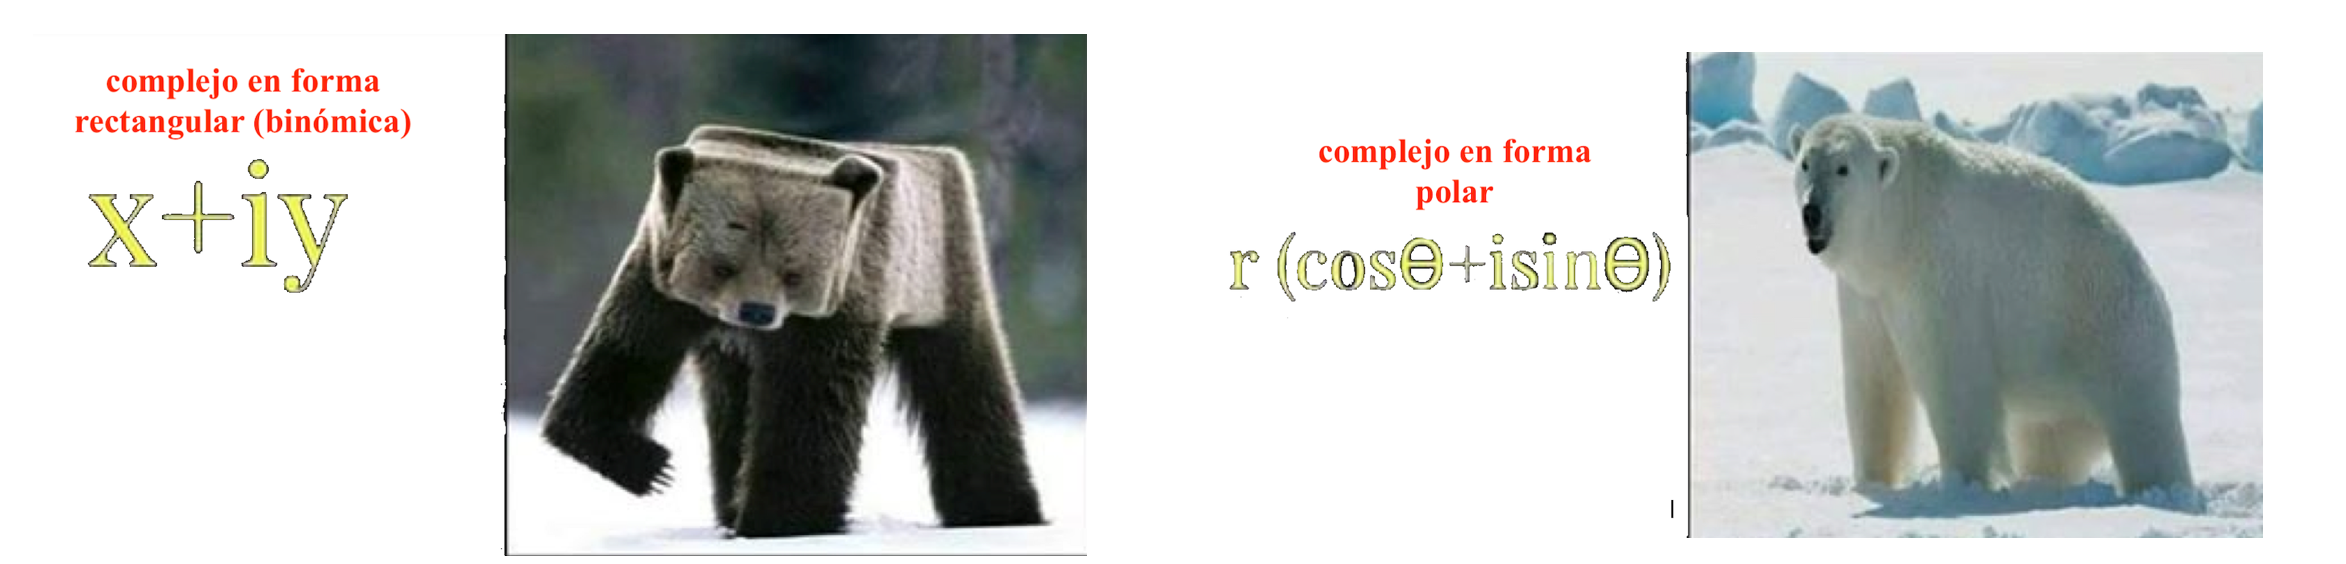
\includegraphics[width=1\textwidth]{img-c/comp08h.png}
\end{figure}



\vspace{5mm}
\subsection{Propiedades del conjugado, del módulo y del argumento de un número complejo}

\begin{tikzpicture}
	\fill [left color=red!50, right color=teal!50] (0,0) rectangle (3.5,.01);
	\fill [left color=teal!50, right color=blue!50] (3.5,0) rectangle (7.5,.01);
	\end{tikzpicture}
\vspace{0.5cm}

\begin{theorem}[ Propiedades conjugado módulo  argumento ]
	
	\begin{enumerate}
	\item $\overline{z_1+z_2} \ = \ \bar z_1 + \bar z_2\, ; \qquad \overline{z_1-z_2}	\ = \ \bar z_1 - \bar z_2\, ; \qquad \overline{z_1\cdot z_2}	\ = \ \bar z_1 \cdot \bar z_2\, ; \qquad \overline{\left( \dfrac {z_1}{z_2} \right) }= \dfrac{\bar z_1}{\bar z_2}$
	\item $arg(\bar z)=-agr(z)$	
	\item $z\ = \bar z \ \leftrightarrow \ z\in \mathbb R$
	\item $|\bar z|\ = \ |z|\, ; \qquad |z_1\cdot z_2|\ = \ |z_1|\cdot |z_2|\, ; \qquad \left| \dfrac {z_1}{z_2} \right| \ = \ \dfrac {|z_1|}{|z_2|}$	
	\item $\Re(z) \ = \ \dfrac{z+\bar z}{2} \, ; \qquad \Im(z) \ = \ \dfrac{z-\bar z}{2\, i} $
	\end{enumerate}

\end{theorem}

\underline{Demostración}: al ser tan sencillas, se dejan como ejercicio para el/la lector/a.


\vspace{5mm}
\subsection{Producto de complejos y giros}

\begin{tikzpicture}
	\fill [left color=red!50, right color=teal!50] (0,0) rectangle (3.5,.01);
	\fill [left color=teal!50, right color=blue!50] (3.5,0) rectangle (7.5,.01);
	\end{tikzpicture}

\vspace{5mm}
	
\begin{figure}[H]
	\centering
	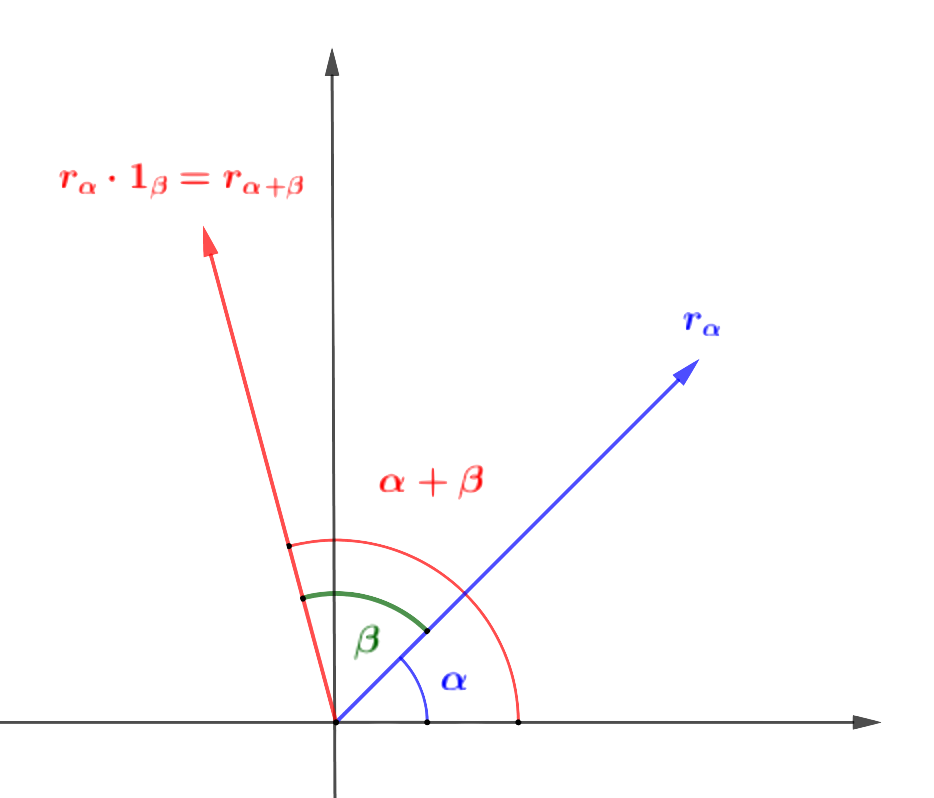
\includegraphics[width=0.5\textwidth]{img-c/comp09.png}
\end{figure}
\vspace{2mm} Al multiplicar un número complejo $z=r_\alpha$ por $1_\beta$ se obtiene el mismo número complejo $z$ pero girado un ángulo $\beta$ respecto del origen de coordenadas.

\begin{myexampleblock}{Aplicaciones geométricas del producto de números complejos}
\begin{figure}[H]
	\centering
	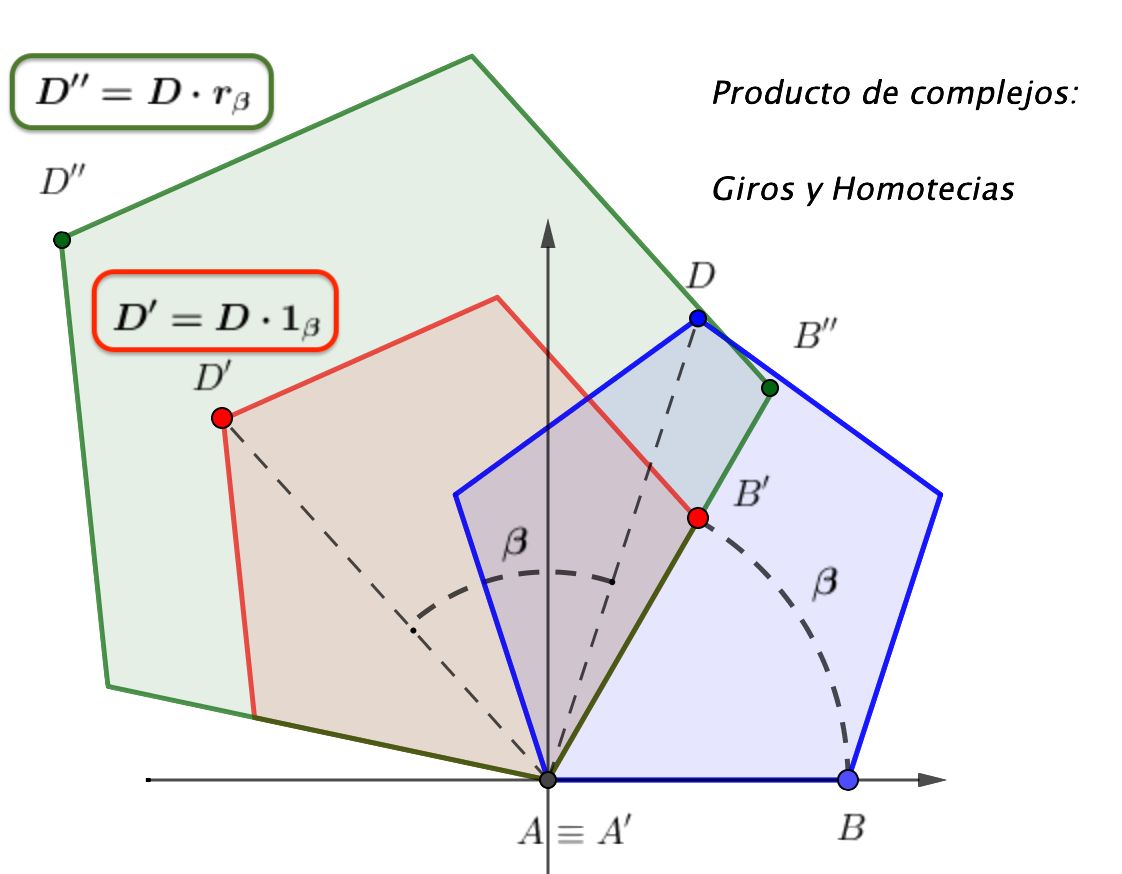
\includegraphics[width=0.75\textwidth]{img-c/comp10.png}
\end{figure}
\end{myexampleblock}	

\vspace{5mm}
\begin{miejercicio}

Uno de los vértices de	un cuadrado centrado en el origen es $A(3,1)$, encuentra las coordenadas de los otros vértices.

\rule{250pt}{0.5pt}

\vspace{2mm} 
\begin{multicols}{2}
Los vértices de un cuadrado, respecto de su centro, forman ángulos de $90^o$; así, al multiplicar $A$ por $1_{\, 90^o}$ obtendremos $B$, el vértice $C$ será $B\cdot 1_{\, 90^o}$ y el $D=C\cdot 1_{\, 90^o}$. 

\vspace{2mm} Supongamos que estamos en el plano complejo, $A\to z_a=3+i$, como, en este caso $1_{\, 90^o}=\boldsymbol i$, multiplicar cada vértice por $1_{\, 90^o}$ es multiplicar por $\boldsymbol i$, luego,

\begin{figure}[H]
	\centering
	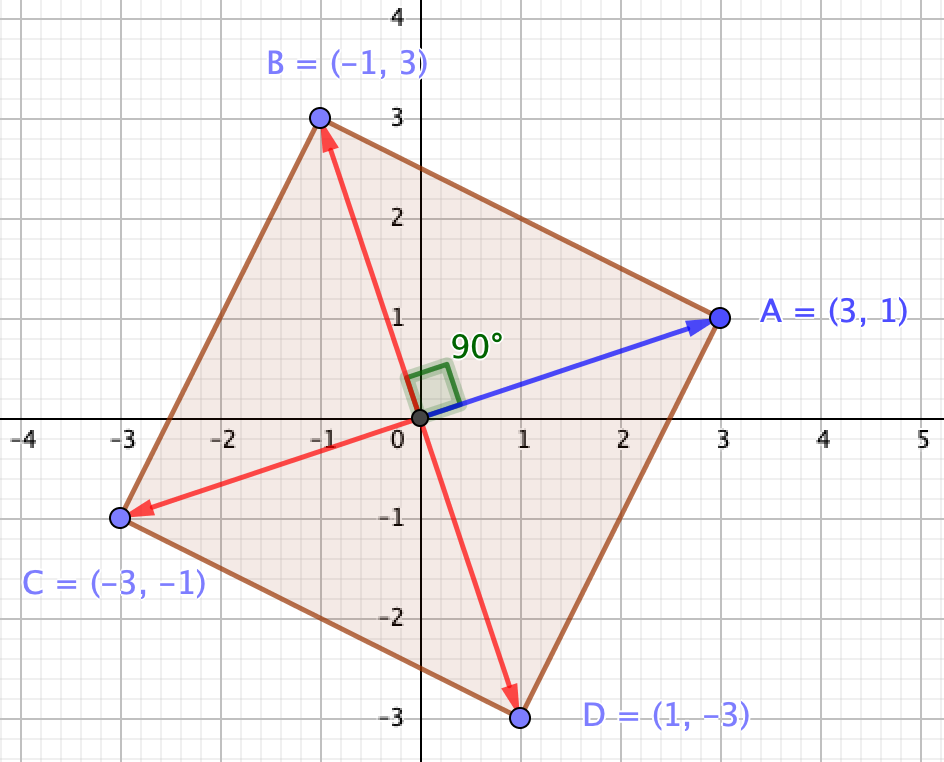
\includegraphics[width=0.45\textwidth]{img-c/comp11.png}
\end{figure}
\end{multicols}
$A=(3,1) \to z_A=3+i;\qquad z_B=z_A\cdot 1_{\, 90^o}=z_A \cdot i =(3+i)\cdot i=3\, i+i^2=-1+3\ i \to B=(-1,3)$

\vspace{2mm} $B=(-1,3) \to z_B=-1+3\, i;\qquad z_C=z_B \cdot i =(-1+3\, i)\cdot i=-i+3\, i^2=-3- i \to C=(-3,-1)$

\vspace{2mm} $C=(-3,-1) \to z_C=-3- i;\qquad z_D=z_C \cdot i =(-3-i)\cdot i=-3i-i^2=1-3\, i \to D=(1,-3)$
\end{miejercicio}

		

\vspace{1cm}
\section{Potencias en $\mathbb C$}

\begin{tikzpicture}
	\fill [left color=red!50, right color=teal!50] (0,0) rectangle (3.5,.1);
	\fill [left color=teal!50, right color=blue!50] (3.5,0) rectangle (7.5,.1);
	\end{tikzpicture}
\vspace{0.5cm}

\begin{theorem}[ Potencias de números complejos]

$$\subrayado{ \boxed{\  \boldsymbol{ (\, r_{\, \alpha} \,)^n \ = \ r^n_{\ \  n\cdot \alpha} } \ }} \ \ , \ \qquad \forall n \in \mathbb N$$

La potencia enésima de un número complejo $z=r_\alpha$ es un número complejo cuyo módulo es la potencia enésima del módulo y cuyo argumento es n-veces el argumento.
	
\end{theorem}

\underline{Demostración}:

$(r_\alpha)^2=r_\alpha \cdot r_\alpha=r^2_{\ 2\alpha};\qquad 
(r_\alpha)^3=(r_\alpha)^2 \cdot r_\alpha=r^2_{\ 2\alpha}\cdot r_\alpha=r^3_{\ 3\alpha};\qquad \cdots \cdots \to$

\hspace{2cm} $ \to \qquad 
\boldsymbol{ (r_\alpha)^n \ = } \ (r_\alpha)^{n-1} \cdot r_\alpha=r^{n-1}_{\ (n-1)\alpha}\cdot r_\alpha=r^n_{\ [n+(n-1)]\alpha} \ \boldsymbol{ = \ r^n_{\ n\, \alpha} }$ \QED

\textcolor{gris}{Para ser rigurosos, a esta demostración es necesaria someterla al \emph{método de inducción}. Se incluirá en un apéndice.}


\vspace{5mm}

\begin{myalertblock}{Potencias complejas de exponente entero}

$z^{-n}=\dfrac 1{z^n}=\dfrac 1{(r_\alpha)^n}=\dfrac{1}{r^n_{\ n\alpha}}	=
\dfrac{1}{r^n(\cos n\alpha + i \sin n\alpha)} = $

\vspace{2mm} $=\dfrac{1}{r^n(\cos n\alpha + i \sin n\alpha)} \cdot \dfrac{\cos n\alpha - i \sin n\alpha}{\cos n\alpha - i \sin n\alpha} = r^{-n} \ \dfrac{ \cos n\alpha - i \sin n\alpha}{\cos^2 n\alpha + \sin^2 n\alpha}=$

\vspace{2mm}$=
r^{-n} \left(\,  \cos(-n\alpha)+i \sin (-n\alpha) \, \right) = r^{-n}_{\ -n\alpha} \quad \Rightarrow \quad \boldsymbol{ (r_\alpha)^{-n} \ = \ r^{-n}_{\ -n\alpha} }$

$$\text{Luego } \qquad \subrayado{ \boxed{ \ \boldsymbol{ (r_\alpha)^n \ = \ r^n_{\ n\alpha} \ , \ \ \ \forall n \in \mathbb Z }  \ } } $$
\end{myalertblock}


\subsection{Fórmula de \emph{Moivre}}

\begin{tikzpicture}
	\fill [left color=red!50, right color=teal!50] (0,0) rectangle (3.5,.01);
	\fill [left color=teal!50, right color=blue!50] (3.5,0) rectangle (7.5,.01);
	\end{tikzpicture}
\vspace{0.5cm}

\begin{theorem}[ Fórmula de Moivre]

$$ \subrayado{ \boxed{ \ \boldsymbol{ ( \, \cos \theta \ + \ i\ \sin \theta \, )^n \ = \ \cos n\theta \ + \ i \sin n\theta  } \ } }  \ \ ; \ \qquad \forall n\in \mathbb Z$$	
\end{theorem}

\underline{Demostración}: basta aplicar la fórmula de potenciación al número $1_\alpha$, en forma trigonométrica.

En efecto, $\ \ (1_\alpha)^n=1_{\, n\alpha} \ \to \ $ en forma trigonometrica, $\quad (\cos \theta +i\, \sin \theta \, )^n  =  \cos n\theta + i\,  \sin n\theta $ \QED

Esta fórmula es de mucha utilidad a la hora de escribir las razones trigonométricas de los ángulos múltiplos enteros de $\alpha$ en función de senos y cosenos de $\alpha$.

\begin{miejercicio}

En el ejercicio 9.1.a vimos que $\ (1+i)^4=-4$, compruébalo ahora con la potenciación de números complejos.

\rule{250pt}{0.5pt}

\vspace{4mm} Primero pasemos a polares $1+i=\mqty[ r=\sqrt{1^1+1^2}=\sqrt{2} \\ \ \alpha=\atan \dfrac 1 1 \to \alpha=45^o \ \scriptsize{\text{(1-cdte)}} \ ]= \sqrt{2}_{\, 45^o}$

\vspace{2mm} Haciendo la potencia, $(1+i)^4=(\sqrt{2}_{\, 45})^4=(\sqrt{2})^4_{\ 45\cdot 4}=4_{\, 180^o}=-4$
\end{miejercicio}

\begin{miejercicio}

Escribe el seno y coseno del ángulo $4\alpha$ en función de los senos y cosenos de $\alpha$

\vspace{2mm} \textcolor{gris}{ Ver ejercicio 7.6 }

\rule{250pt}{0.5pt}

\vspace{2mm} Por la fórmula de Moivre: $(1_\alpha)^4=1_{\, 4\alpha} \quad \to \quad (\cos \alpha+i\sin \alpha)^4=\cos 4\alpha+i\sin 4\alpha$

\vspace{2mm}$\underline{ \cos 4\alpha+i\sin 4\alpha }= (\cos \alpha+i\sin \alpha)^4 = \cos^4 \alpha + 4 \cos^3 \alpha \, i \sin \alpha + 6 \cos^2 \alpha \, i^2 \sin^2 \alpha + 4 \cos \alpha \, i^3 \sin^3 \alpha + i^4 \sin^4 \alpha=\cos^4 \alpha + 4 \cos^3 \alpha \, i \sin \alpha - 6 \cos^2 \alpha  \sin^2 \alpha - 4 \cos \alpha \, i \sin^3 \alpha +  \sin^4 \alpha= \underline{(\, \cos^4 \alpha -6\cos^2 \alpha \sin^2 \alpha +\sin^4 \alpha \, ) \ + \ i\, (\, 4\cos^3 \alpha \sin \alpha -4\cos \alpha \sin^3 \alpha \, )}$

\vspace{2mm} Identificando partes reales e imaginarias, $\quad \begin{cases}
 \ \boldsymbol{ \cos 4\alpha = \cos^4 \alpha -6\cos^2 \alpha \sin^2 \alpha +\sin^4 \alpha } \\ \ \boldsymbol{ \sin 4\alpha =  4\cos^3 \alpha \sin \alpha -4\cos \alpha \sin^3 \alpha } \end{cases}$
 
 \vspace{2mm} \textcolor{gris}{(Se ha usado el desarrollo de la potencia 4 del binomio de Newton)}

	
\end{miejercicio}


\vspace{1cm}
\section{Radicación en $\mathbb C$}

\begin{tikzpicture}
	\fill [left color=red!50, right color=teal!50] (0,0) rectangle (3.5,.1);
	\fill [left color=teal!50, right color=blue!50] (3.5,0) rectangle (7.5,.1);
	\end{tikzpicture}
\vspace{0.5cm}


\begin{theorem}[ Raíz n-sima de un número complejo]

$$\subrayado{\boxed{ \ \boldsymbol{ 
\sqrt[n]{ \, r_{\, \alpha} \, } 
\ = \ \left( \sqrt[n]{\, r \, } \right)_{\ \dfrac{\alpha + 360\cdot k}{n} } \ }} }\ ; \qquad \forall k \in \underbrace{\{0,1,2,\cdots , n-1\}}_{n-\text{valores}}$$

La raíz $n$-sima de un número complejo es un complejo cuyo módulo es la raíz n-sima del módulo y argumento igual al que tenía más $k$ vueltas ($360^o$), dividido por $n$; donde $k\in \{0,1,2,\cdots, n-1\}$. \textbf{Así, la raíz $n$-sima de un complejo tiene $\boldsymbol n$ soluciones distintas.}
	
\end{theorem}

\underline{Demostración}:  $\quad $ Sea $\ \  z=r_\alpha \quad \to \quad \sqrt[n]{z}=z'=s_\beta \in \mathbb C \ / \ z\ =\ \boldsymbol{ r_\alpha} \ = \ (z')^n \  = \ (s_\beta)^n \ =\ \boldsymbol{ s^n_{\ n\cdot \beta}} \quad \Rightarrow$

Conocemos $r$ y $\alpha$ y pretendemos hallar $s$ y $\beta$, identificando módulos y argumentos,

$\Rightarrow \begin{cases}
 \ r=s^n &\to \quad s=\sqrt[n]{r}	 \\
 \ \alpha=n \cdot \beta &\to \quad \beta=\dfrac{\alpha+360\cdot k}{n}\ ; \ \ k\in \{0,1,2,\cdots, n-1\}
 \end{cases}$ \QED

\vspace{4mm}
\begin{miejemplo}

Hallar las raíces cúbicas de la unidad.
\begin{multicols}{2}
$\sqrt[3]{1}=\sqrt[3]{1_{\, 0^o}}\ = \ \sqrt[3]{1}_{\ \dfrac{0+360\, k}{3}}=1_{\, 120\, k} \ $

Con $\quad k\in \{0,1,2\} \quad \to \quad $

$\to \ \ \sqrt[3]{1} \ = \ \begin{cases}
 \ 1_{\, 0^o} &= 1 \\ \ 1_{\, 120^o} &= -\dfrac 1 2 +\dfrac{\sqrt{3}}{2}\, i 	\\ \ 1_{\, 240^o} &= -\dfrac 1 2 -\dfrac{\sqrt{3}}{2}\, i 
 \end{cases}$
 
 \vspace{2mm} En $\mathbb R$ la raíz cúbica de la unidad tiene una solución, en $\mathbb C$ tiene tres. 
 	
\begin{figure}[H]
	\centering
	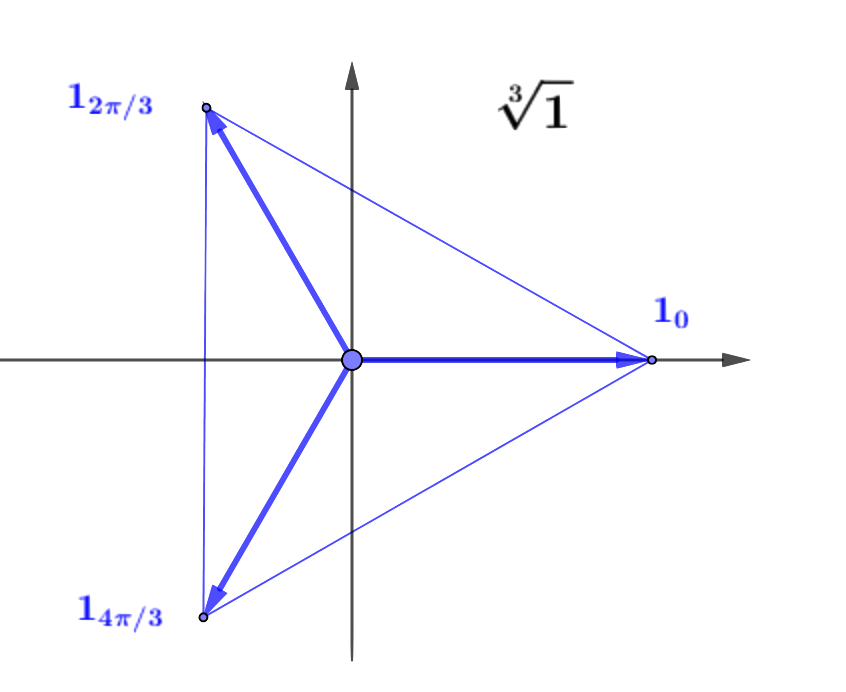
\includegraphics[width=0.5\textwidth]{img-c/comp12.png}
\end{figure}
\end{multicols}
Los afijos de las soluciones son los vértices de un triángulo equilátero.
\end{miejemplo}


\begin{miejercicio}

Calcula: $\quad \sqrt{5+12\, i}$

\rule{250pt}{0.5pt}

\vspace{2mm} $\triangleright \ \ $ En forma polar:	

\vspace{2mm} $5+12\, i\  = \ \left[ \mqty{ r=\sqrt{5^2+12^2}=13 \\ \alpha=\atan 12/5=67.38^o \ \scriptsize{\text{(1-cdte)}}} \right] \ = \ 13_{\, 67.38^o}$

\vspace{2mm} $\sqrt{5+12\, i} = \sqrt{13_{\, 67.38}}= 3.61_{\  \dfrac{67.38+360\, k}{2}  }=3.61_{\ 33.675+180\, k}\ ; \ \ k\in\{0,1\} \ \ \to $

\vspace{2mm} $\to \begin{cases} \ k=0 &\to \ 3.61_{\, 33.675}\ =\ 3\ +2\, i \\ \ k=1 &\to \ 3.61_{\, 213.675}=-3-2\, i\end{cases}$


\vspace{4mm} $\triangleright \ \ $ En forma binómica  \textcolor{gris}{(solo con raíces cuadradas)}:	

\vspace{2mm}  $\sqrt{5+12\, i}=a+b\, i \ \leftrightarrow \ 5+12\, i=(a+b\, i)^2=a^2-b^2+2ab\, i \ \to $

\vspace{2mm} $\to \ \begin{cases} \ 5&=a^2-b^2 \\ \ 12&=2ab \end{cases} \ \to \quad \cdots \quad \to \ \ \begin{cases} \ a=3\, , \ b=2 \\ a=-3\, , \ b=-2 \end{cases}$ $\quad \Rightarrow \quad $  $\ 3+2\, i \ $ y $ \ -3-2\, i$

\end{miejercicio}


\begin{miejercicio}

Una de las raíces quintas de un número complejo es $2\, i$. Calcula cuál es ese número y cuales son las otras raíces y represéntalas en el diagrama de Argand (plano complejo). Calcula también el área del pentágono que forman las raíces y el perímetro.

\rule{250pt}{0.5pt}

\begin{multicols}{2}
$\sqrt[5]{z}=2\, i=2_{\, 90^o} \ \to \ z=(2_{\, 90^o})^5=32_{\, 450}=32_{\, 90^o}=32\, i$

\vspace{2mm} $\sqrt[5]{32_{90}}=(\sqrt[5]{32})^5_{\ \dfrac{90+360\, k}{5}}=2_{\ 18+72\, k}$

\vspace{2mm} Con $\ \ k\in \{0,1,2,3,4\}$

\vspace{2mm} $\sqrt[5]{32_{\, 90^o} } \ = \ 2_{\, 18^o};\ \ 2_{\, 90^o};\ \ 2_{\, 162^o};\ \ 2_{\, 234^o};\ \ 2_{\, 306^o}  $
 
 \vspace{2mm} El área del pentágono es la de 5 triángulos isósceles de lados iguales de $l=2\, $ u y ángulo comprendido de $\theta=72^o$, el lado opuesto lo obtenemos por el \emph{teorema del coseno}:
 

\begin{figure}[H]
	\centering
	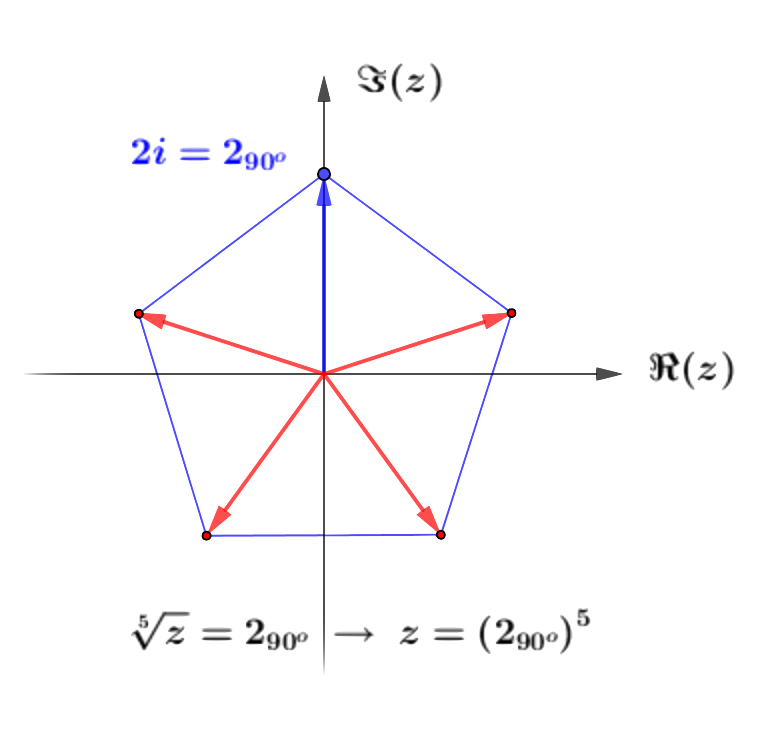
\includegraphics[width=0.5\textwidth]{img-c/comp13.png}
\end{figure}	
\end{multicols}
$x^2=2^2+2^2-2\cdot 2\cdot 2 \cdot \cos 72 \ \to \ x=2.35\, $ u. El perímetro será $\mathcal P=5\, x= 11.76\, $ u y el área, $\mathcal A=\frac 1 2\, l\, l\, \sin \theta=\frac 1 2\, 2\, 2\ \sin 72^o=1.90\, $ u$^2$.
	
\end{miejercicio}

\underline{Observaciones} de la radicación en $\mathbb C$:

Como $\ \sqrt[n]{ \, r_{\, \alpha} \, } 
\ = \ \left( \sqrt[n]{\, r \, } \right)_{\ \frac{\alpha + 360\cdot k}{n} } \ $, la diferencia angular entre raíces (diferencia de fase) es de $\frac {360}{n}$, por ello, las soluciones forman un polígono regular de $n$ lados y ángulos centrales  $\frac {360}{n}$.



\vspace{1cm}
\begin{myalertblock} {Forma exponencial de un número complejo}
	
	En cálculo se demostrará que $\ \  \boldsymbol{e^{\, i\, \theta} \ = \ \cos \theta \ + \ i\, \sin \theta} \ , \ \ $ por lo que podremos escribir un número complejo como:
	
	
$$\subrayado{ \boxed{\ 
\boldsymbol{z 
\ = \  
\underbrace {\ a \ + \ b\, i \ }_{\text{ forma binómica }} 
\ = \ 
\underbrace{\ r_{\ \theta} \ }_{\text{ forma polar }} 
\ = \ 
\underbrace{\ r\, (\cos \theta \ + \ i\, \sin \theta) \ }_{\text{ forma trigonométrica } } 
\ = \ 
\underbrace {r\, e^{\, i \, \theta} }_{ \text{ forma exponencial } }
} \ } }$$

Siguiendo esta forma de escritura de números complejos, Euler encontró la \emph{\textbf{fórmula más hermosa}}:

$$-1=1_{\pi}=e^{\, i\, \pi} \quad \Rightarrow \qquad \large{ \subrayado{\boxed{\ \boldsymbol{ e^{\, i \, \pi} \ + \ 1 \ = \ 0 } \ } }  } $$

Expresión que involucra al cero, la unidad, el número e y la unidad imaginaria, todo ello en una sencilla, simple y hermosa fórmula.

\begin{figure}[H]
	\centering
	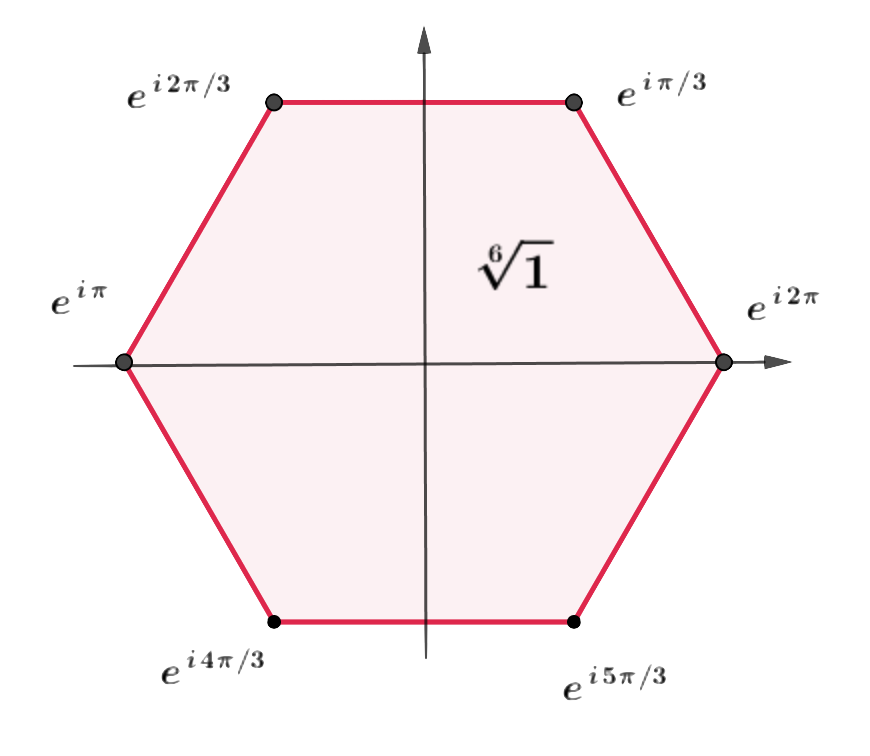
\includegraphics[width=0.6\textwidth]{img-c/comp14.png}
\end{figure}

\end{myalertblock}


\vspace{5mm}
\begin{myalertblock}{Funciones trigonométricas complejas: funciones hiperbólicas}

$\left. { \mqty{e^{iz}=\cos z+i\sin z\\ e^{-iz}=\cos(-z)+i\sin(-z)=\cos z-i\sin z\ \ } } \right\} \ \Rightarrow \ \begin{cases}
\quad \cos z=\dfrac{e^{i\, z}+e^{-i\, z}}{2} 	\\ \quad \sin z=\dfrac{e^{i\, z}-e^{-i\, z}}{2i}
 \end{cases}$	
 
\vspace{2mm} Para $z\in \mathbb R$ las fórmulas proporcionan el seno y coseno ordinarios, pero si  $z$ es un número imaginario puro $\ z \ \to \ i\, x$:

\vspace{2mm} $\begin{cases}
\quad \cos i\, x=\dfrac{e^{i^2x}+e^{-i^2x}}{2}= \dfrac{e^{-x}+e^x}{2}& = \quad \boldsymbol{
\dfrac{ e^x+e^{-x} }{2} 
} \boldsymbol{=\ \cosh x}	\\ 
\quad \sin i\, x=\dfrac{e^{i^2x}-e^{-i^2x}}{2i}=\dfrac{-e^{x}+e^{-x}}{2i} & =\quad \boldsymbol{i \, \dfrac{e^x-e^{-x}}{2} } \boldsymbol{=\sinh x}
 \end{cases}$
 
 \vspace{2mm} que son el seno y cosenos hiperbólicos \textcolor{gris}{(estos conceptos se verán en ampliación de cálculo)}
 
 \vspace{2mm} \textsf{!`En forma exponencial, el argumento siempre en radianes!}
\end{myalertblock}



\vspace{1cm}
\section{Ecuaciones y sistemas en $\mathbb C$}

\begin{tikzpicture}
	\fill [left color=red!50, right color=teal!50] (0,0) rectangle (3.5,.1);
	\fill [left color=teal!50, right color=blue!50] (3.5,0) rectangle (7.5,.1);
	\end{tikzpicture}
\vspace{0.5cm}

Las ecuaciones y sistemas en $\mathbb C$ se tratarán como en $\mathbb R$ pero teniendo en cuenta que la raíz enésima de un complejo tiene exactamente $n$ soluciones.

\begin{theorem}[ Teorema fundamental del álgebra]

\emph{Todo polinomio de grado $n$ de una variable (con grado mayor que cero) con coeficientes complejos tiene, contando las multiplicidades, exactamente $n$ raíces complejas.}	
\end{theorem}

\begin{miejemplo}

Resuelve la ecuación: $\ \ x^{5} - 7 \; x^{4} + 25 \; x^{3} - 35 \; x^{2} - 16 \; x + 52 = 0$

\vspace{4mm} Probando por los divisores del término independiente por Ruffini, rápidamente encontramos que $2$ es una raíz doble y $-1$ una raíz simple	 y podremos escribir:

\vspace{2mm} $x^{5} - 7 \; x^{4} + 25 \; x^{3} - 35 \; x^{2} - 16 \; x + 52 = (x-2)^2\, (x+1)\, (x^2-4x+3) = 0$

\vspace{2mm} Resolviendo la ecuación de segundo grado encontramos $\ x^2-4x+3 = 0 \ \leftrightarrow \ x=2\pm 3\, i$, dos soluciones más, por lo que podemos escribir:

\vspace{2mm}  $x^{5} - 7 \; x^{4} + 25 \; x^{3} - 35 \; x^{2} - 16 \; x + 52 = (x-2)^2\, (x+1)\, (x-(2+3i))\, (x-(2-3i)) = 0 \ \to $

\vspace{2mm} $\to \ \begin{cases}
\  (x-2)^2=0 &\to  x=2 \ \text{ raíz real doble (2)} \\
\  (x+1)=0 &\to   x=-1 \ \text{ raíz real simple (1)} \\
\ (x-(2+3i))=0 &\to x=2+3i \ \text{ raíz compleja simple (1)}  \\ 
\ (x-(2-3i))=0 &\to  x=2-3i \ \text{ raíz compleja simple (1)}	
 \end{cases}$

\vspace{2mm} Polinomio grado $5$ que tiene efectivamente $(2)+(1)+(1)+(1)=5$ soluciones, contando las multiplicidades.

\end{miejemplo}


\vspace{2cm}
\begin{multicols}{2}
\section{Ejercicios}

\begin{tikzpicture}
	\fill [left color=red!50, right color=teal!50] (0,0) rectangle (3.5,.1);
	\fill [left color=teal!50, right color=blue!50] (3.5,0) rectangle (7.5,.1);
	\end{tikzpicture}

$\quad$

\vspace{5mm} $\quad$

\begin{figure}[H]
	\centering
	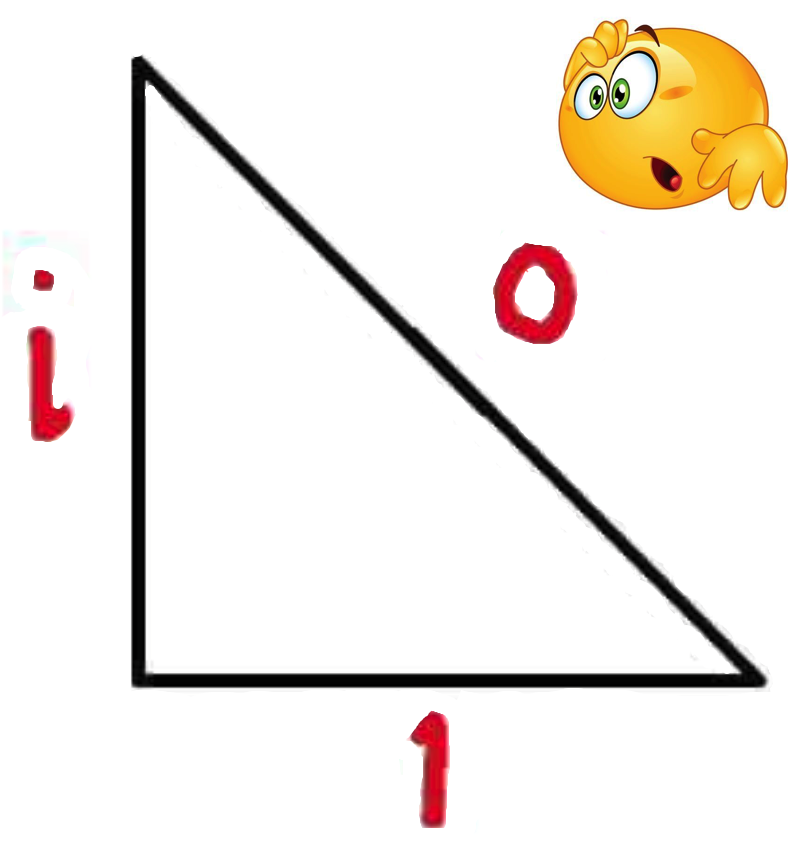
\includegraphics[width=0.2\textwidth]{img-c/comp07.png}
\end{figure}
\end{multicols}
\vspace{0.5cm}

%%%%%
\begin{miejercicio}

Calcula: $\qquad \dfrac{(3-2\, i)^2 - (1+i)\, (2-i)}{-3+i}$

\rule{250pt}{0.5pt}

\vspace{4mm} $\dfrac{(3-2\, i)^2 - (1+i)\, (2-i)}{-3+i}= \dfrac{(9-12\, i+4\, i^2 )- (2-i+2\, i-i^2)}{-3+i}= \dfrac{(5-12\, i)-(3+i)}{-3+i}=$

\vspace{2mm} $=\dfrac{2-13\, i}{-3+i}\cdot \dfrac{-3-i}{-3-i}=\dfrac{-6-2\, i +39\, i +13\, i^2}{(-3)^2-i^2}=\dfrac{-19+37\, i}{10}=-\dfrac{19}{10}+\dfrac{37}{10}\, i$


\end{miejercicio}

%%%%%
\begin{miejercicio}

Determina $\ a \ $ y $\ b \ $ para que $\quad 5(a-2\, i)\ = \ (3+i)\, (b-i)$

\rule{250pt}{0.5pt}

\vspace{2mm} $ 5(a-2\, i)\ = \ (3+i)\, (b-i) \ \to \ 5a-10\, i=3b-3\, i +b\, i -i^2 \ \to \ 5a\ -\ 10\, i \ = \ (3b+1) \ + \ (b-3)\, i\ \Rightarrow$

\vspace{2mm} $\Rightarrow \ \begin{cases} \ \ 5a = 3b+1 \\ -10 = b-3 \end{cases} \ \Rightarrow \quad  b=-7 \ \ \wedge \ \ a=-4$

\end{miejercicio}

%%%%%
\begin{miejercicio}

Sea $\ z=\dfrac{3-2x\, i}{4+3\, i}\, , \  $ determina el valor de $\ x\in \mathbb R\ $ para que
$\quad$ a) $\ z\ $ sea imaginario puro; $\quad$ b) $\ z\ $ sea un número real.

\rule{250pt}{0.5pt}

\vspace{4mm} $z=\dfrac{3-2x\, i}{4+3i}=\dfrac{3-2x\, i}{4+3\, i}\dfrac{4-3\, i}{4-3\, i}=\dfrac{}{4^2-3^2\, i^2}=\dfrac{12-9\, i-8x\, i+6x\, i^2}{25} = \dfrac{12-6x}{25}-\dfrac{9+8x}{25}\, i$

\vspace{4mm} $\triangleright\ \ a)\quad z$ es imaginario puro si $\Re(z)=0 \ \to \ \dfrac{12-6x}{25}=0 \ \to 12-6x=0 \ \Rightarrow \ x=2$

\vspace{2mm} $\triangleright\ \ b)\quad z$ es un número real si $\Im(z)=0 \ \to \ -\dfrac{9+8x}{25}=0 \ \to \ 9+8x=0 \ \Rightarrow \ x=-9/8$


\end{miejercicio}

%%%%%
\begin{miejercicio}

Determina el valor de $\ x \ $ para que $\ \ \dfrac{x+i}{2+i} \ $ tenga por módulo $2$.

\rule{250pt}{0.5pt}

\vspace{2mm} $\dfrac{x+i}{2+i} = \dfrac{x+i}{2+i} \cdot \dfrac{2-i}{2-i}=\dfrac{2x+2\, i -x\, i -i^2}{2^2-i^2} =\dfrac{(2x+1) \ + \ (2-x)\, i}{5}= \dfrac{2x+1}{5}+\dfrac{2-x}{5}\, i$

\vspace{2mm} $r=\sqrt{\left(\dfrac{2x+1}{5}\right)^2+\left(\dfrac{2-x}{5}\right)^2}= \dfrac{ \sqrt{ (4x^2+4x+1)\ + \ (4-4x+x^2) } }{5}=\dfrac{\sqrt{5x^2+5}}{5}=2 \ \Rightarrow$

\vspace{2mm} $ \sqrt{5x^2+5}=10 \ \to \ 5x^2+5=100 \ \to \ 5x^2=95 \ \to x^2=19 \ \to \ |x|=\sqrt{19} \ \Rightarrow \ $ 

\vspace{2mm} $\Rightarrow \ \  x=\sqrt{19} \ \ \vee \ \ x=-\sqrt{19}$

\end{miejercicio}

%%%%%
\begin{miejercicio}

Encuentra dos números complejos tales que su cociente sea $\ 2_{\, 150^o} \ $ y su producto $\ 18_{\, 90^o}$

\rule{250pt}{0.5pt}

\vspace{2mm} Sean $\ r_\alpha$ y $s_\beta$ los números buscados,
$\ \to \ \begin{cases}
\ r_\alpha \div s_\beta=(r/s)_{\, \alpha-\beta}= 2_{\, 150}  
&\to \ \begin{cases} \ r/s&=2 \\ \ \alpha-\beta&=150   \end{cases}
\\ \\
\ r_\alpha \cdot s_\beta=(r\cdot s)_{\, \alpha+\beta}=18_{\, 90}	
&\to \ \begin{cases}  r\cdot s &=18 \\ \ \alpha+\beta&=90  \end{cases}
\end{cases}$

\vspace{2mm} $\begin{cases} \ r/s&=2 \\ \ r\cdot s&=18 \end{cases} \ \to \ \cdots \ \to \ r=6\ \ \wedge \ \ s=3 $

\vspace{2mm} $\begin{cases} \ \alpha-\beta&=150 \\ \ \alpha+\beta=90 \end{cases} \ \to \ \cdots \ \to \ \alpha=300^o \ \ \wedge \ \ \beta=150^o$

\vspace{2mm} Los números buscados son $\ 6_{\, 300^o} \ $ y $ \ 3_{\, 150^o}$



\end{miejercicio}

%%%%%
\begin{miejercicio}

Calcula $\qquad \dfrac
{ (-1+i)^4 \ (\sqrt{3}-i) }
{ i^{20} \ \left( -\dfrac 1 2+\dfrac{\sqrt{3}}{2} \ i  \right) }$

\rule{250pt}{0.5pt}

\vspace{2mm} Como hay  productos, cocientes y potencias, trabajaremos en forma polar.

\vspace{2mm} $\triangleright \quad  -1+i =\  \left[ \mqty{ r=\sqrt{(-1)^2+1^2}=\sqrt{2} \\ \alpha=\atan \frac {1}{-1} = 135 \  \tiny{\text{(2-cdte)}} } \right] \ = \sqrt{2}_{\ 135^o}\, ; \quad (-1+i)^4=\left ( \sqrt{2}_{\ 135^o} \right)^4= 4_{\, 540}=4_{\, 180^o} $

\vspace{2mm}  $\triangleright \quad  \sqrt{3}-i = \ 
\left[ 
\mqty{ 
r=\sqrt{ (\sqrt{3})^2+(-1)^2 } 
\\ 
\alpha=\atan \frac{-1}{\sqrt{3}} = \atan (- \frac{\sqrt{3}}{3}) = 330 \ \tiny{\text{(4-cdte) }}
} 
\right] \ = 2_{\, 330^o}$

\vspace{2mm}  $\triangleright \quad  i^{20} = (i^4)^5=1^5=1=1_{\, 0^o}$

\vspace{2mm}  $\triangleright \quad   -\dfrac 1 2+\dfrac{\sqrt{3}}{2} \ i  = \ 
\left[
\mqty{
r=\sqrt{\left(-\frac 1 2 \right)^2 + \left( \frac{\sqrt{3}}{2} \right)^2 } = 1 
\\
\alpha=\atan \frac{\sqrt{3}/2}{-1/2}=\atan -\sqrt{3}=120 \ \tiny{\text{(2-cdte) }}
}
\right] \ 
= 1_{\, 120^o}$

\vspace{2mm} $\dfrac
{ (-1+i)^4 \ (\sqrt{3}-i) }
{ i^{20} \ \left( -\dfrac 1 2+\dfrac{\sqrt{3}}{2} \ i  \right) } = 
\dfrac{4_{\, 180} \cdot 2_{\, 330}}{1_{\, 0} \cdot 1_{\, 120}}=\dfrac{8_{\, 510}}{1_{\, 120}}=8_{\, 390}=8_{\, 30^o}=8(\cos 30^o+i\, \sin 30^o)=4\sqrt{3}+4\, i$

\end{miejercicio}



%%%%%
\begin{miejercicio}

El punto $(-2,0)$ es un vértice de un triángulo equilátero centrado en el origen. Calcula los otros vértices, el perímetro y el área del triagulo.

\rule{250pt}{0.5pt}

\vspace{2mm} Si $(-2,0)$  es un vértice, el afijo del número complejo que hemos de considerar es $-2=2_{\, 180^o}$ y los tres vértices serán las raíces cúbicas de un número complejo $z$ de las que una de ellas es $2_{\, 180^o}$

\vspace{2mm} Busquemos $z$ y las otras dos raíces que serán los otros dos vértices. 

\vspace{2mm} $\sqrt[3]{z}=2_{\, 180^o} \ \to z=(2_{\, 180^o})^3=8_{540}=8_{\, 180^o}=-8$ 

\vspace{2mm} $\sqrt[3]{8_{180}} = 2_{\, \frac{180+360\, k}{3} } = 
2_{60+120k}=
\begin{cases}  \ k=0 &\to \ 2_{\, 60^o} \\  \ k=1 &\to \ 2_{\, 180^o} \\  \ k=2 &\to \ 2_{\, 300^o} \end{cases}$ 

\vspace{2mm}  En geometría analítica se demuestra que la distancia entre dos puntos del plano, $(x_1,y_1)$ y $(x_2,y_2)$ es $d=\sqrt{(x_2-x_1)^2+(y_2-y_1)^2}$, por lo que, tomando las coordenadas (forma binómica) de dos vértices (afijos de las raíces cúbicas), encontraremos el lado $l$ del triángulo. Es evidente que el ángulo comprendido entre dos lados de un triángulo equilátero es siempre $60^o$. 

\vspace{2mm} $2_{180}=-2+0i\to (-2,0)=(x_1,y_1); \quad 2_{60}=2\cos 60+i\, \sin 60=1+\sqrt{3}\, i\to (1,\sqrt{3})=(x_2,y_2)$

\vspace{2mm} $l=d=\sqrt{(1-(-2)^2+(\sqrt{3}-0)^2}=\sqrt{9+3}=2\sqrt{3}$ u

\vspace{2mm} Perímetro: $\ \mathcal P=3\cdot l=6\sqrt{3}\ \mathrm{u};\quad$  Área: $\ \mathcal A=\frac 1 2\,  l^2 \sin \theta=\dfrac 1 2 \cdot (2\sqrt{3})^2 \, \sin 60 = 3\sqrt{3}\ \mathrm{u}^2$


\end{miejercicio}

%%%%%
\begin{miejercicio}

Los afijos de dos números reales y de dos imaginarios puros forman un cuadrado centrado en el origen de área 6 u$^2$. ?`De qué número son raíces cuartas?

\rule{250pt}{0.5pt}


\begin{multicols}{2}
Llamemos $\ x,\ -x,\ x\, i \text{ y } -x\, i \ $ a estos afijos (números complejos) que serán la raíz cuarta del número pedido, $x=\sqrt[4]{z} \ \to \ z=x^4$

\vspace{2mm}Al ser el área del cuadrado 6 u$^2$, el lado del mismo será $\ l=\sqrt{6}$ u y la diagonal $\ d=\sqrt{2} l = \sqrt{2} \sqrt{6} = 2\sqrt{3}$ u. Por lo que $\ x=\sqrt{3}$ u, como muestra la siguiente figura.

\vspace{2mm} Los vértices (afijos) del cuadrado son $\sqrt{3},\ -\sqrt{3},\ \sqrt{3}\, i  \text{ y } -\sqrt{3}\, i$
\begin{figure}[H]
	\centering
	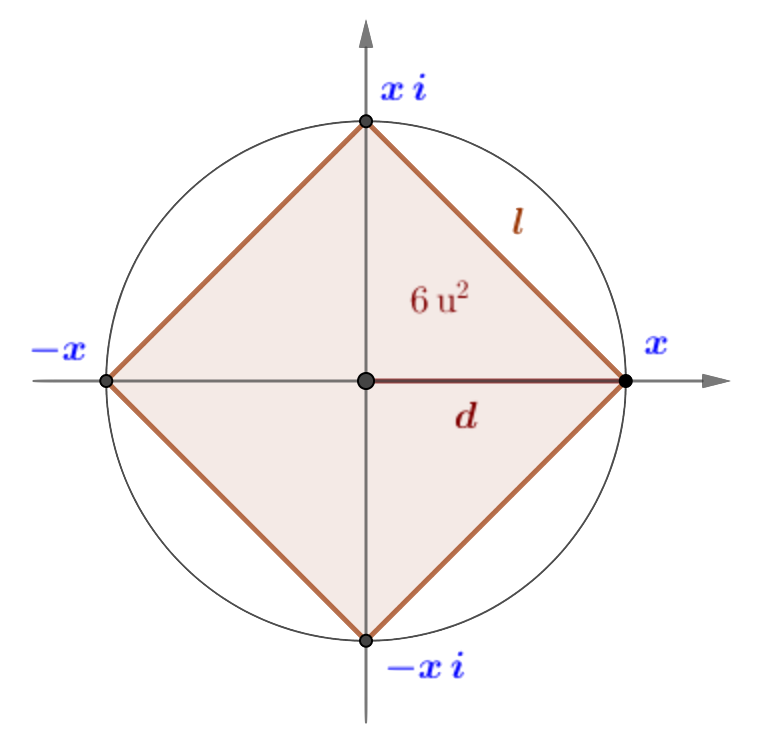
\includegraphics[width=0.4\textwidth]{img-c/comp15.png}
\end{figure}	
\end{multicols}

\vspace{2mm} Como, por ejemplo, $\ \sqrt[4]{z}=\sqrt{3}_{0} \ \to \ z=(\sqrt{3}_{0})^4=9_{\, 0^o}= 9$. El número buscado es $\boldsymbol 9$

\end{miejercicio}


%%%%%
\begin{miejercicio}

Resuelve el sistema de ecuaciones complejas: $\qquad \begin{cases} \ 2z+w&=8+i\\ \ z+i\, w&=1-i \end{cases}$

\vspace{2mm}

\rule{250pt}{0.5pt}

\vspace{2mm} Multiplicando la segunda ecuación por dos y restándole la primera:

\vspace{2mm} $(-1+2\, i)\, w =-6-3\, i \ \to \ w=\dfrac{-6-3\, i}{-1+2\, i} \cdot \dfrac{-1-2\, i}{-1-2\, i}=\dfrac{6+12\, i+3\, i+6\, i^2}{(-1)^2-2^2\, i^2}=\dfrac{15\, i}{5}=3\, i$

\vspace{2mm} Sustituyendo en la segunda ecuación:
$\quad z+i\, (3\, i)=1-i \ \to z-3=1-i º \to \ z=4-i$
\end{miejercicio}


%%%%%
\begin{miejercicio}

Resuelve las ecuaciones: $\qquad a)\ z^6+64=0\, ; \qquad \qquad b)\ z^4+(1+i)z^2+5i=0$ 

\rule{250pt}{0.5pt}

\vspace{6mm} $\triangleright \ \ a)\quad z^6=-64=64_{\, 180^o} \ \to \ z=\sqrt[6]{64_{180}}=2_{\frac{180+360k}{6}}=2_{30+60k}=
\begin{cases}
\ k=0 &\to \ 2_{\, 30^o} \\
\ k=1 &\to \ 2_{\, 90^o}=2\, i \\	
\ k=2 &\to \ 2_{\, 150^o} \\
\ k=3 &\to \ 2_{\, 210^o} \\
\ k=4 &\to \ 2_{\, 270^o}=-2\, i \\
\ k=5 &\to \ 2_{\, 330^o} 
\end{cases}$

\vspace{10mm} $\triangleright \ \ b)\quad z^4+(1+i)\, z^2+5i=0\ $ Bicuadrada, \underline{cambio}: $\boldsymbol{z^2=w} \ \to \ w^2+(1+i)\, w+5i=0$

\vspace{2mm} $w^2+(1+i)\, w+5i=0 \ \to \ w=\dfrac{-(i+1)\pm \sqrt{(-1+i)^2-4\cdot 1\cdot 5i}}{2\cdot 1}=\dfrac{(-1+i)\pm \sqrt{-18\, i}}{2} \ (*)$

\vspace{2mm} $\sqrt{-18\, i}=\sqrt{18_{270}}=3\sqrt{2}_{\frac{270+360k}{2}}=3\sqrt{2}_{135+180k}=$

\vspace{2mm} $=\begin{cases}
\ 3\sqrt{2}_{135}=3\sqrt{2} (\cos 135+i\, \sin 135)=3\sqrt{2} \left( -\dfrac{\sqrt{2}}{2} +i\, \dfrac{\sqrt{2}}{2} \right)=-3+3\, i	
\\
\ 3\sqrt{2}_{315}=3\sqrt{2} (\cos 315+i\, \sin 315)=3\sqrt{2} \left( \dfrac{\sqrt{2}}{2} -i\, \dfrac{\sqrt{2}}{2} \right)=3-3\, i=-(-3+3\, i)	
\end{cases}$

\vspace{2mm} Luego $\ (*) \ \ w=\dfrac{(-1+i)\pm (-3+3\, i)}{2} = \begin{cases}
 \ w_1=\dfrac{-4+2\, i}{2}=-2+i = \ \sqrt {5}_{\,153.43^o}\\
 \ w_2=\dfrac{2-4\, i}{2}=1-2\, i =\ \sqrt{5}_{\ 296.57^o}	
 \end{cases}$


\vspace{2mm} Hay que \underline{deshacer el cambio}: $\quad z^2=w \ \to \ z=\sqrt{w}\,, \ $ dos soluciones en cada caso.

\vspace{2mm} $z=\sqrt{-2+i}=\sqrt{\sqrt{5}_{153.43}}=\sqrt[4]{5}_{\dfrac{153.43+360k}{2}}=\sqrt[4]{5}_{76.72+180k}=\begin{cases}
\ z_1=\sqrt[4]{5}_{\ 76.72^o}	 \\ \ z_2=\sqrt[4]{5}_{\ 256.72^o} \end{cases}$

\vspace{2mm} $z=\sqrt{1-2\, i}=\sqrt{\sqrt{5}_{296.57}}=\sqrt[4]{5}_{\dfrac{296.57+360k}{2}}=\sqrt[4]{5}_{128.36+180k}=\begin{cases}
\ z_1=\sqrt[4]{5}_{\ 128.36^o}	 \\ \ z_2=\sqrt[4]{5}_{\ 308.36^o} \end{cases}$


\end{miejercicio}

%****************
\vspace{10mm}%****
%****************

%%%%%%%%%%%%%%
\begin{mipropuesto}

Calcula $\qquad \dfrac{3\, i^{774}+i^{2027}}{1+i^{3125}}$	
\end{mipropuesto}

\vspace{-8mm}
\begin{flushright}
\begin{footnotesize} \textcolor{gris}{\rotatebox{180}{ -2+i }}	\end{footnotesize}
\end{flushright}


%%%%%%%%%%%%%%
\begin{mipropuesto}

Determina $x$ e $y$ para que $\quad \dfrac{3-x\, i}{1+2\, i}\ = \ y+2\, i$	
\end{mipropuesto}

\vspace{-8mm}
\begin{flushright}
\begin{footnotesize} \textcolor{gris}{\rotatebox{180}{ x=-16, y=7 }}	\end{footnotesize}
\end{flushright}


%%%%%%%%%%%%%%
\begin{mipropuesto}

Determina el valor de $k$ para que $\ \ \dfrac{1+k\, i}{3-4\, i} \ $ sea a) un número real;  b) sea un número imaginario puro; y c) esté en la bisectriz del primer y tercer cuadrantes.	
\end{mipropuesto}

\vspace{-8mm}
\begin{flushright}
\begin{footnotesize} \textcolor{gris}{\rotatebox{180}{ a) -4/3; b) 3/4; c) (birectriz: parte real=parte imaginaria) -1/7}}	\end{footnotesize}
\end{flushright}


%%%%%%%%%%%%%%
\begin{mipropuesto}

Dados los complejos $2-a\, i$ y $3-b\, i$, halla $a$ y $b$ para que su producto sea igual a $8+4\ i$.
\end{mipropuesto}

\vspace{-8mm}
\begin{flushright}
\begin{footnotesize} \textcolor{gris}{\rotatebox{180}{ $a=2/3 \ \wedge \ b=3 \quad \vee \quad a=-2 \ \wedge \ b=1$ }}	\end{footnotesize}
\end{flushright}


%%%%%%%%%%%%%%
\begin{mipropuesto}

Sean: $\quad z_1=3-2\, i;\quad z_2=-3+i;\quad z_3=5\, i \ $ Calcular:

$a)\ \ z_1+2z_2-z_3;\quad b)\ \ z_1(z_2+z_3)+z_3;\quad c) \ \ (z_1+2z_3)\, (z_2-z_1);\quad d)\ \ 5\,\dfrac{z_2-z_1}{z_3}$	
\end{mipropuesto}

\vspace{-8mm}
\begin{flushright}
\begin{footnotesize} \textcolor{gris}{\rotatebox{180}{ $a)\ \ -3-5\, i;\quad b)\ \ 3+29\, i;\quad c)\ \ -42-39\, i;\quad d)\ \ 3+6\, i$ }}	\end{footnotesize}
\end{flushright}


%%%%%%%%%%%%%%
\begin{mipropuesto}

Calcula las 10 primeras potencias del número $1+i$ y represéntalas, ?`qué figura se obtiene?	
\end{mipropuesto}

\vspace{-8mm}
\begin{flushright}
\begin{footnotesize} \textcolor{gris}{\rotatebox{180}{ Una espiral. }}	\end{footnotesize}
\end{flushright}

%%%%%%%%%%%%%%
\begin{mipropuesto}

Calcula y da el resultado en forma binómica: $\quad a)\ \ (-1- i)^5	\, ; \qquad b)\ \ (2\sqrt{3}+2\, i)^6$
\end{mipropuesto}

\vspace{-8mm}
\begin{flushright}
\begin{footnotesize} \textcolor{gris}{\rotatebox{180}{ $a)\ \ 4+4\, i\, ; \qquad b)\ \ -4096$ }}	\end{footnotesize}
\end{flushright}

%%%%%%%%%%%%%%
\begin{mipropuesto}

Calcula $\ \sqrt[4]{-16} \ $ y da el resultado en forma binómica.	
$\ \ $ Lo mismo para $\ \sqrt[3]{\dfrac{2-2\, i}{-3+3\, i}}$
\end{mipropuesto}

\vspace{-8mm}
\begin{flushright}
\begin{footnotesize} \textcolor{gris}{\rotatebox{180}{ $\pm \sqrt{2}\pm \sqrt{2}\, i;\qquad \pm \sqrt{2/3}\, i$ }}	\end{footnotesize}
\end{flushright}

%%%%%%%%%%%%%%
\begin{mipropuesto}

Calcula $\ \sqrt[3]{\dfrac{1+i^{501}}{1+i^{743}}} \ $ y da el resultado en forma binómica.
\end{mipropuesto}

\vspace{-8mm}
\begin{flushright}
\begin{footnotesize} \textcolor{gris}{\rotatebox{180}{ $\frac 1 2+\frac{\sqrt{3}}{2}\, i ;\ \ -1;\ \ \frac 1 2-\frac{\sqrt{3}}{2}\, i$  }}	\end{footnotesize}
\end{flushright}


%%%%%%%%%%%%%%
\begin{mipropuesto}

Calcula las razones trigonométricas de los ángulos de $15^0$ y de $105^o$
\end{mipropuesto}

\vspace{-8mm}
\begin{flushright}
\begin{footnotesize} \textcolor{gris}{\rotatebox{180}{ $\sin 15 = (\sqrt{6}-\sqrt{2})/2;\ \ \cos 15 = (\sqrt{6}+\sqrt{2})/2 ;\quad \sin 105 = (\sqrt{2} +\sqrt{6})/2;\ \ \cos 105 = (\sqrt{2} -\sqrt{6})/2$  }}	\end{footnotesize}
\end{flushright}

\vspace{-10mm}
\begin{flushright}
\begin{footnotesize} \textcolor{gris}{\rotatebox{180}{ $1_{45} \div 1_{30}=1_{15};\ \ 1_{60}+1_{45}=1_{105} $  }}	\end{footnotesize}
\end{flushright}


%%%%%%%%%%%%%%
\begin{mipropuesto}

Escribe el seno y coseno de $3\theta$ en función del seno y coseno de $\theta$
\end{mipropuesto}

\vspace{-8mm}
\begin{flushright}
\begin{footnotesize} \textcolor{gris}{\rotatebox{180}{ $(1_\theta)^3=1_{3\theta}\qquad \sin 3 \theta= 3\cos^2 \theta \sin \theta - \sin^3 \theta;\ \ \ \cos 3\theta= \cos^3\theta-3\sin^2 \theta \cos \theta$ }}	\end{footnotesize}
\end{flushright}





\vspace{-8mm}
\begin{flushright}
\begin{footnotesize} \textcolor{gris}{\rotatebox{180}{ $(-0.91, 1.78)\, , \ (-1.97, -0.31)\, , \  (-0.31, -1.97)\, , \  (1.78, -0.91) \ ; \qquad l=2.6\ \mathrm{u}$ }}	\end{footnotesize}
\end{flushright}


%%%%%%%%%%%%%%
\begin{mipropuesto}

Busca dos números complejos cuya suma sea $-3 + 3\, i$ y que una de las raíces cuadradas de su cociente sea $2\, i$.
\end{mipropuesto}

\vspace{-8mm}
\begin{flushright}
\begin{footnotesize} \textcolor{gris}{\rotatebox{180}{ $1-i \ \ \text{ y } \ \ -4+4\, i$  }}	\end{footnotesize}
\end{flushright}


%%%%%%%%%%%%%%
\begin{mipropuesto}

Encuentra el número complejo cuyo cuadrado coincide con su conjugado.
\end{mipropuesto}

\vspace{-8mm}
\begin{flushright}
\begin{footnotesize} \textcolor{gris}{\rotatebox{180}{ (Trabaja en polares, $\ (r_\alpha)^2=\overline{r_\alpha}=r_{-\alpha}) \qquad 0,\ \ 1_0,\ \ 1_{120},\ \ 1_{240}$   }}	\end{footnotesize}
\end{flushright}

%%%%%%%%%%%%%%
\begin{mipropuesto}

La suma de dos complejos es $3+i$, la parte real del primero es $2$ y el cociente de éste entre el segundo es un número real. Determina esos números.
\end{mipropuesto}

\vspace{-8mm}
\begin{flushright}
\begin{footnotesize} \textcolor{gris}{\rotatebox{180}{ $2+\frac 2 3 \, i \ \text{ y } \ 1+\frac 1 3 \, i$  }}	\end{footnotesize}
\end{flushright}


%%%%%%%%%%%%%%
\begin{mipropuesto}

Encuentra dos números complejos cuyo producto sea $8\, i$, la diferencia de sus argumentos sea $\pi/6$ y la suma de sus módulos sea 6.
\end{mipropuesto}

\vspace{-8mm}
\begin{flushright}
\begin{footnotesize} \textcolor{gris}{\rotatebox{180}{ (Trabaja en forma polar) $\qquad 2_{60} \ \text{ y } \ 4_{30} \quad \text{ ó } \quad 4_{60} \ \text{ y } \ 2_{30} $   }}	\end{footnotesize}
\end{flushright}

%%%%%%%%%%%%%%
\begin{mipropuesto}

Un pentágono regular con centro en el origen de coordenadas tiene uno de sus vértices en el punto $(\sqrt 2,\, \sqrt 2)$. Halla los otros vértices y la longitud de su lado.
\end{mipropuesto}

%%%%%%%%%%%%%%
\begin{mipropuesto}

$-2\, i\ $ es una de las raíces sextas de cierto número complejo, ?`cuál?. Determina las otras raíces.
\end{mipropuesto}

\vspace{-8mm}
\begin{flushright}
\begin{footnotesize} \textcolor{gris}{\rotatebox{180}{ El número buscado es $-64$. Las raíces son $\ 2_{45+60\cdot k};\ \ k\in\{0,1,2,3,4,5\} $  }}	\end{footnotesize}
\end{flushright}


%%%%%%%%%%%%%%
\begin{mipropuesto}

Calcula la longitud y el área de un cuadrado centrado en el origen cuyos vértices son los afijos de las raíces de la ecuación $\ z^4+16=0$

\end{mipropuesto}

\vspace{-8mm}
\begin{flushright}
\begin{footnotesize} \textcolor{gris}{\rotatebox{180}{ $l=2\sqrt 2$ u; $\qquad \mathcal A=8  $ u$^2$  }}	\end{footnotesize}
\end{flushright}


%%%%%%%%%%%%%%
\begin{mipropuesto}

El afijo de $3 + 2\, i$ es uno de los vértices de un cuadrado con centro en el origen de coordenadas. Halla los otros vértices y el área del cuadrado.
\end{mipropuesto}

\vspace{-8mm}
\begin{flushright}
\begin{footnotesize} \textcolor{gris}{\rotatebox{180}{ $(-2, 3);\ (-3, -2) \text{ y }  (2, -3); \quad \mathcal A=26 $u$^2$  }}	\end{footnotesize}
\end{flushright}



%%%%%%%%%%%%%%
\begin{mipropuesto}

Encuentra una ecuación cuyas raíces sean $\ 1, \ 1-3\, i,\ -1,\ 1+3\, i$
\end{mipropuesto}

\vspace{-8mm}
\begin{flushright}
\begin{footnotesize} \textcolor{gris}{\rotatebox{180}{ (Factoriza) $\qquad z^4-2z^3+9z^2+2z-10=0$ }}	\end{footnotesize}
\end{flushright}


%%%%%%%%%%%%%%
\begin{mipropuesto}

Resuelve los siguientes ecuaciones en $\ \mathbb C$

\begin{multicols}{3}
\begin{enumerate}[a) ]
	\item $\ z^4+2z^2+2=0$
	\item $\ z^4+(1-\sqrt{3}\, i)=0$
	\item $\ z^6+7z^3-8=0$
\end{enumerate}	
\end{multicols}

\end{mipropuesto}

\vspace{-8mm}
\begin{flushright}
\begin{footnotesize} \textcolor{gris}{\rotatebox{180}{ $a)\ \pm 4,\ \pm 4i;\quad b)\ 2_{60},\ 2_{180},\ 2_{300};\quad c)\ 1_o,\ 1_{120},\ 1_{240};\ 2_{60},\ 2_{180},\ 2_{300}$ }}	\end{footnotesize}
\end{flushright}


%%%%%%%%%%%%%%
\begin{mipropuesto}

Resuelve: $\quad a)\ \ \begin{cases} \ 2z-5w=-5+2\, i \\ \ 4z-3w=-3-10\, i \end{cases} \qquad \qquad b)\ \ \begin{cases} \ z+w=-1+2\, i \\ \ i\, z+(1-i)\, w = 1+3\, i \end{cases}$
\end{mipropuesto}

\vspace{-8mm}
\begin{flushright}
\begin{footnotesize} \textcolor{gris}{\rotatebox{180}{ $a)\ \ w=1-2\, i;\ \ z=-4\, i;\qquad b)\ \ z=0;\ \ w=-1+2\, i$ }}	\end{footnotesize}
\end{flushright}


\vspace{1cm}

\begin{myalertblock}{Descripción gráfica en $\boldsymbol{ \mathbb C }$}

\begin{figure}[H]
	\centering
	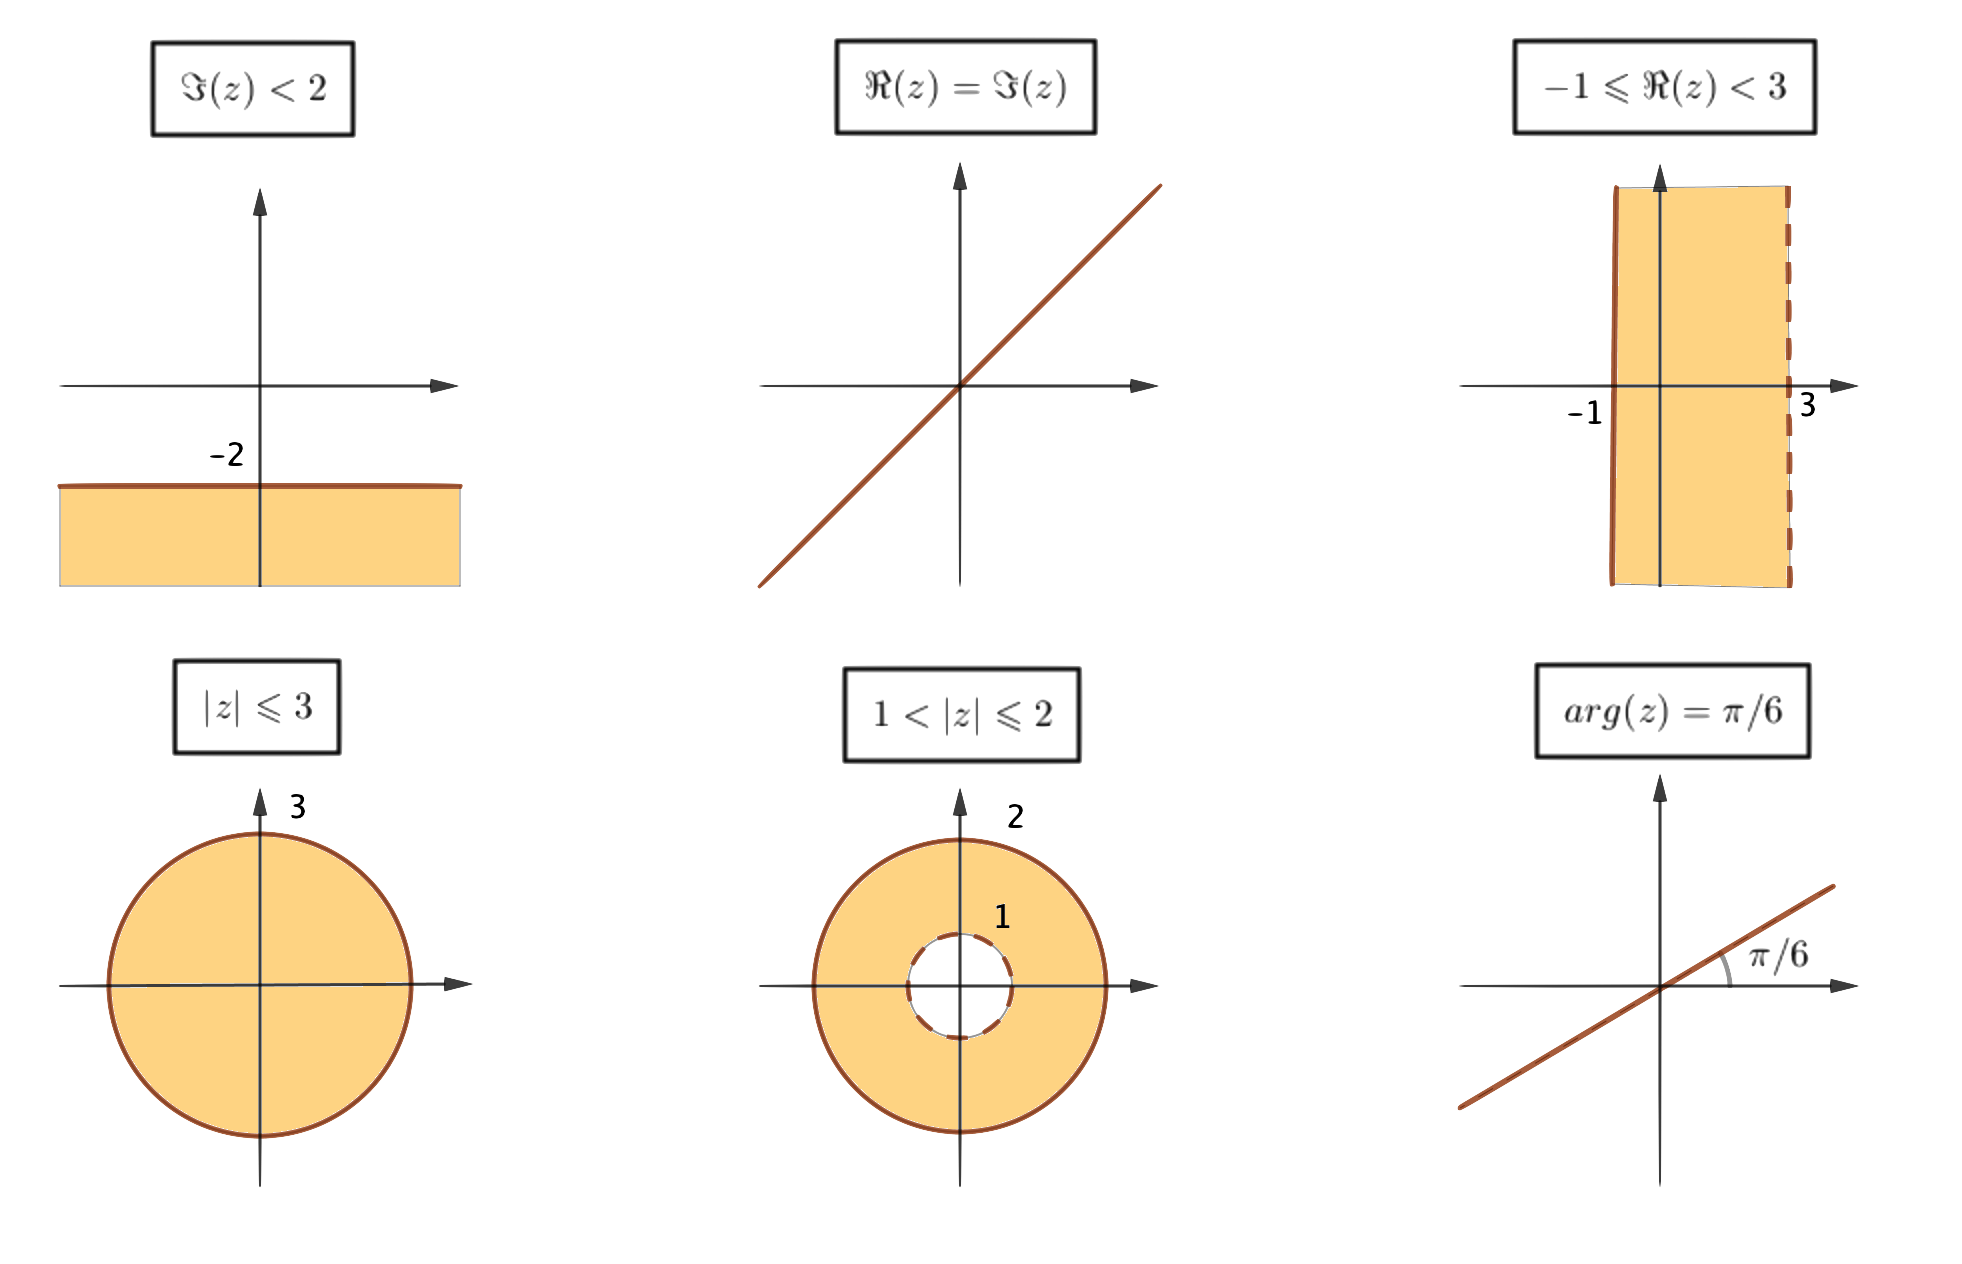
\includegraphics[width=1\textwidth]{img-c/comp16.png}
\end{figure}
	
\end{myalertblock}




%++++++++++++++++++++++++++++++++++++
%********************************************************************
%\newpage
\vspace{3cm} %%%%%%%%%%%%%%%%%%%%%%%
\begin{adjustwidth}{50pt}{250pt}
\begin{cuadro-naranja}
\textbf{\huge{Problemas $\boldsymbol{+}$}}\normalsize{$\, $}
\end{cuadro-naranja}	
\end{adjustwidth}

\vspace{5mm}
\begin{enumerate}[\textbf{P$\boldsymbol +$} 1. ]

%%%%
\item	Calcula, en función de $n$, $\quad i+i+i^2+i^3+\cdots +i^n$ 

\vspace{-6mm}
\begin{flushright}
\begin{footnotesize} \textcolor{gris}{\rotatebox{180}{ (suma PG) $\quad 	\dfrac{1-i^{n+1}}{1-i}; \qquad 1 \ si \ n=\ 	\dot{4};\ \ 1+i \ si \  n=\dot 4+1;\ \ i \ si \ n=\dot 4+2;\ \ 0 \ si \ n=\dot 4+3 $}}	\end{footnotesize}
\end{flushright}

%%%%
\item	?`Qué falla en el siguiente razonamiento?

$$ (-1)\, (-1) \ = \ 1\, ; \quad \sqrt{(-1)\, (-1)} \ = \ \sqrt{1}\, ; \quad \sqrt{-1}\, \sqrt{-1} \ = \ 1 \, ; \quad i^2 \ = \ 1 \, ; \quad \boxed{ \ \boldsymbol{-1\ = \ 1} \ }$$

\vspace{-6mm}
\begin{flushright}
\begin{footnotesize} \textcolor{gris}{\rotatebox{180}{ $\sqrt{a\cdot b}=\sqrt{a}\cdot \sqrt{b} \quad \Leftrightarrow \quad \sqrt{a}>0 \ \wedge \ \sqrt{b}>0 $ }}	\end{footnotesize}
\end{flushright}

%%%%
\item	Los afijos de dos números complejos conjugados junto al origen de coordenadas determinan un triángulo. Determina esos números sabiendo que el triángulo es equilátero y que su área es $3\sqrt{3}$ u$^2$.

\vspace{-6mm}
\begin{flushright}
\begin{footnotesize} \textcolor{gris}{\rotatebox{180}{ (Equilátero si $\sqrt{a^2+b^2}=2b$;$\ $ área$=1/2\, (2a)\, b$) $\quad \pm 3+\sqrt{3}\, i \ \text{y} \ \pm 3-\sqrt{3}\, i$ }}	\end{footnotesize}
\end{flushright}

%%%%
\item	Calcula $\qquad a)\ \ \left( \dfrac{\sqrt{i}+i\, \sqrt{i}}{i} \right)^2; \qquad b)\ \ \dfrac{(1+i)^{85}}{(1-i)^{83}}$

\vspace{-6mm}
\begin{flushright}
\begin{footnotesize} \textcolor{gris}{\rotatebox{180}{ (tTrabaja en polar) $\quad a)\ \ 2;\qquad b)\ \ 2$ }}	\end{footnotesize}
\end{flushright}

%%%%
\item	Calcula: $\qquad a)\ \ i+i^2+i^3+\cdots +i^{99}+i^{100} \qquad b)\ \ $?`$\, i^{-1}+i^{-2}+i^{-3}+i^{-4}=i+i^2+i^3+i^4 \, ?$

\vspace{-6mm}
\begin{flushright}
\begin{footnotesize} \textcolor{gris}{\rotatebox{180}{ $a)\ \ $ (PG) $\ 0;\qquad b)\ \ $ Sí. }}	\end{footnotesize}
\end{flushright}

%%%%
\item	Calcula la suma de todas las raíces con parte real positiva de $\ x^{12}-64=0$

\vspace{-6mm}
\begin{flushright}
\begin{footnotesize} \textcolor{gris}{\rotatebox{180}{ $2\sqrt{2}+\sqrt{6}$ }}	\end{footnotesize}
\end{flushright}

%%%%
\item	Si $\ z=\frac 1 2+\frac{\sqrt{3}}{2}\, i \ $ es una de las raíces de $z^4+z^2+1=0$, ?`qué vale la suma $\ z^{12}+z^{11}+z^{10}+\cdots +z^2+z+1\, $? 

\vspace{-6mm}
\begin{flushright}
\begin{footnotesize} \textcolor{gris}{\rotatebox{180}{ (Saca $z^4+z^2+1=0$ factor común). $\quad 1 $  }}	\end{footnotesize}
\end{flushright}

%%%%
\item	Si $z\in \mathbb C$, tal que $z^2=2z-2$, calcula $z^4$ 

\vspace{-6mm}
\begin{flushright}
\begin{footnotesize} \textcolor{gris}{\rotatebox{180}{ (Ten en cuenta que $z^2=2z-2$ y calcula $z^4$) $\qquad -4$ }}	\end{footnotesize}
\end{flushright}


\end{enumerate}


\newpage %%%%%%%%%%%%%%%%%%%%%%%%%%%%%%%%%%%%%%%%%%%%

\section{Resumen del tema}

\begin{tikzpicture}
	\fill [left color=red!50, right color=teal!50] (0,0) rectangle (3.5,.1);
	\fill [left color=teal!50, right color=blue!50] (3.5,0) rectangle (7.5,.1);
	\end{tikzpicture}
\vspace{0.5cm}
\begin{myblock}{Resumen \emph{``Números complejos''}}

\vspace{2mm} $$\boldsymbol i\ = \ \sqrt{-1} \quad \Rightarrow \quad i^2=-1;\ \ i^3=-i;\ \ i^4=1 \qquad  \qquad  i^{-n}=(-1)^n \cdot i^n \,  ; \ \ \forall n \in \mathbb N$$

$$ \mathbb C \ = \ \{ \ z\ = \ x \ +\ i\, y \ \ / \ \ x=\Re(z)\, , \ y=\Im(z)\ \in \mathbb R \ \}$$

$$z\ = \ a \ + \ b \,  i \quad \to \quad \overline{\, z\, } \ = \ a \ - \ b\, i \qquad \qquad \qquad \dfrac 1 z \ = \ \dfrac 1 z \cdot \dfrac{\bar z}{\bar z} \ = \  \dfrac{1}{z\cdot \bar z} \ \overline{ \, z \, }$$

\begin{figure}[H]
	\centering
	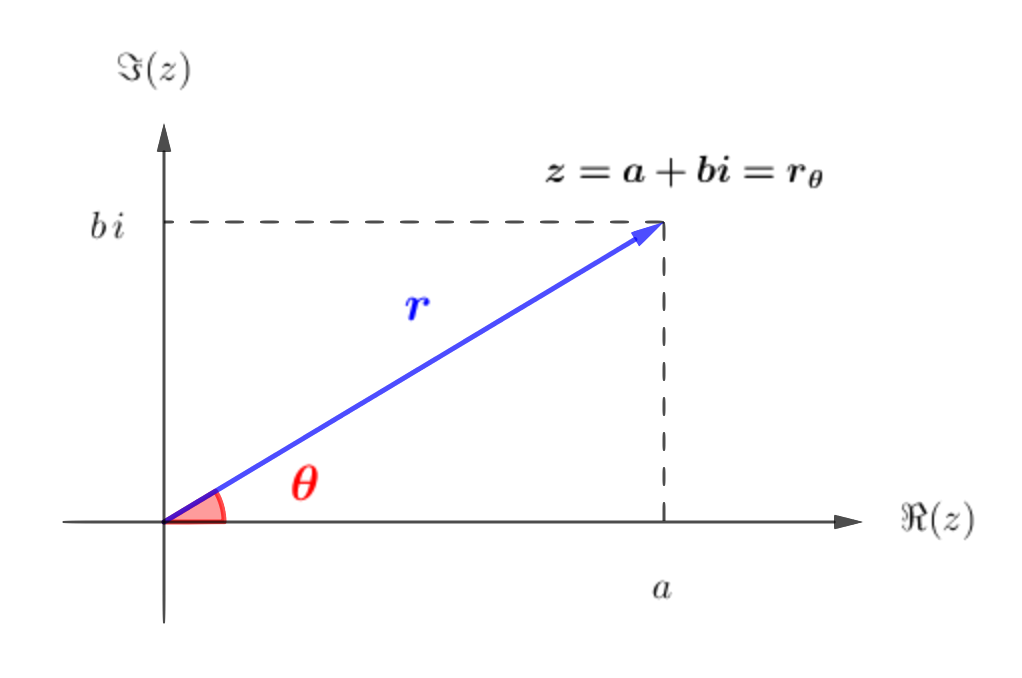
\includegraphics[width=0.5\textwidth]{img-c/comp04.png}
\end{figure}



$$\boxed{\ 
\boldsymbol{z 
\ = \  
\underbrace {\ a \ + \ b\, i \ }_{\text{ forma binómica }} 
\ = \ 
\underbrace{\ r_{\ \theta} \ }_{\text{ forma polar }} 
\ = \ 
\underbrace{\ r\, (\cos \theta \ + \ i\, \sin \theta) \ }_{\text{ forma trigonométrica } } 
\ = \ 
\underbrace {r\, e^{\, i \, \theta} }_{ \text{ forma exponencial } }
} \ } $$

$$r=\sqrt{a^2+b^2}\, ; \qquad \theta=\atan \dfrac b a \qquad \qquad \qquad a=r\cos \theta\, ; \quad b=r\sin \theta$$

$$r_\alpha \cdot s_\beta \ = \ (r\cdot s)_{\, \alpha+\beta} \qquad \dfrac{r_\alpha}{s_\beta}\ = \ \left( \dfrac r s \right)_{\ \alpha-\beta} \qquad (r_\alpha)^n \ = \ (r^n)_{\ n\cdot \alpha}$$

$$ \text{ MOIVRE: } \ (\cos \theta+i\, \sin \theta)^n \ = \ \cos n\, \theta+i\, \sin n\, \theta $$

$$\sqrt[n]{\, r_\theta \ } = \ (\sqrt[n]{r})_{\ \dfrac{\theta+360\cdot k}{n}}\ ; \quad k\in\{0,1,2,\cdots ,n-1\}$$

\vspace{2mm} \emph{Teorema fundamental del álgebra: todo polinomio de grado $n$ de una variable (con grado mayor que cero) con coeficientes complejos tiene, contando las multiplicidades, exactamente $n$ raíces complejas.}	
	
\end{myblock}





\begin{comment}
%%%%%%%%%%%%%%%%%%%%%%%%%%%%%%%%%%%. SECCIONES


\begin{figure}[H]
	\centering
	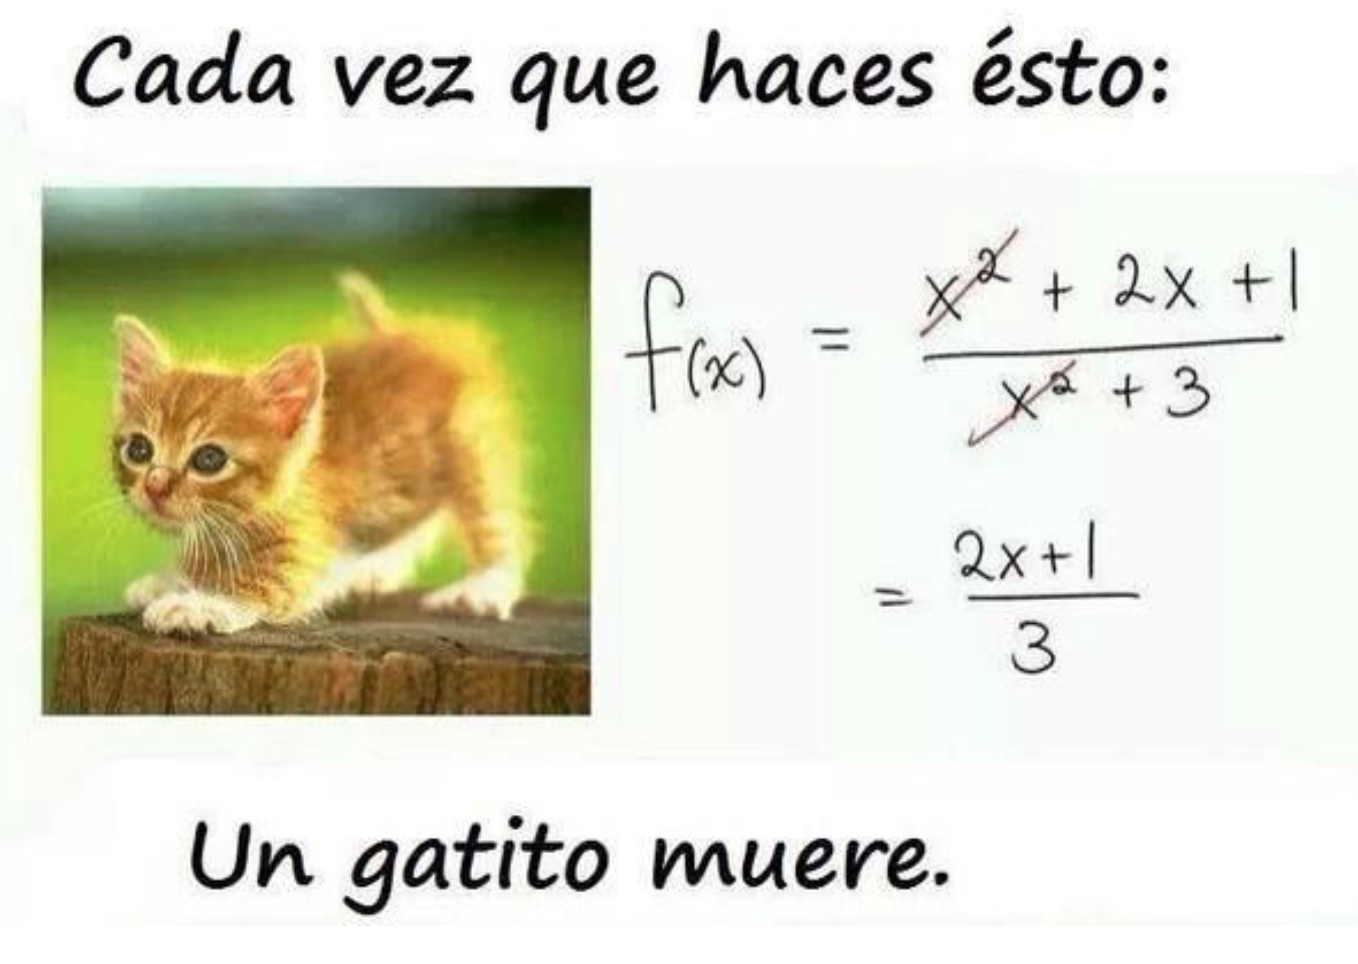
\includegraphics[width=0.35\textwidth]{img-pol/pol05.png}
\end{figure}




\chapter{texto}

\begin{tikzpicture}
	\fill [left color=red!50, right color=teal!50] (0,0) rectangle (6.5,.2);
	\fill [left color=teal!50, right color=blue!50] (6.5,0) rectangle (11.5,.2);
	\end{tikzpicture}

\vspace{1cm}
\section{texto}

\begin{tikzpicture}
	\fill [left color=red!50, right color=teal!50] (0,0) rectangle (3.5,.1);
	\fill [left color=teal!50, right color=blue!50] (3.5,0) rectangle (7.5,.1);
	\end{tikzpicture}
\vspace{0.5cm}

\subsection{texto}

\begin{tikzpicture}
	\fill [left color=red!50, right color=teal!50] (0,0) rectangle (3.5,.01);
	\fill [left color=teal!50, right color=blue!50] (3.5,0) rectangle (7.5,.01);
	\end{tikzpicture}
\vspace{0.5cm}


%%%%%%%%%%%%%%%%%%%%%%%%%%%%%%%%%%%. \begin{ ------>. 
detsacado;  cuadro-naranja;  cuadro-gris;  miejercicio (solución extensa);  mipropuesto (solución corta y fuera del cuadro)

%%%%%%%%%%%%%%%%%%%%%%%%%%%%%%%%%%%. CURIOSIDAD
\vspace{1cm}
\color{ForestGreen!80}
\rule{250pt}{0.2pt}
Texto
\vspace{-8mm}
\begin{flushright}
\rule{250pt}{0.2pt}		
\end{flushright}	
\color{black}
\end{comment}